\section{Podstawy teoretyczne głębokiego uczenia}

\subsection{Głębokie uczenie - podstawowe definicje}

Głębokie uczenie (ang. \emph{deep learning}) jest jedną z~najbardziej dynamicznie rozwijających się gałęzi sztucznej inteligencji (ang. \emph{artificial intelligence}). Zadaniem głębokiego uczenia jest wychwycenie jak największej liczby zależności (cech) występujących w~analizowanym zbiorze danych i~przedstawienie tych zależności w~prostszy sposób - przy pomocy sieci neuronowej z~odpowiednio dobranymi wagami. Głębokie uczenie można sklasyfikować jako podzbiór uczenia reprezentacji (ang. \emph{representation learning}), które z~kolei jest podzbiorem uczenia maszynowego (ang. \emph{machine learning}), a~to w~końcu stanowi podzbiór metod sztucznej inteligencji. Rysunek \ref{fig:diagram1} prezentuje diagram zależności pomiędzy wyżej wymienionymi dziedzinami.

\begin{figure}[!h]
    \centering 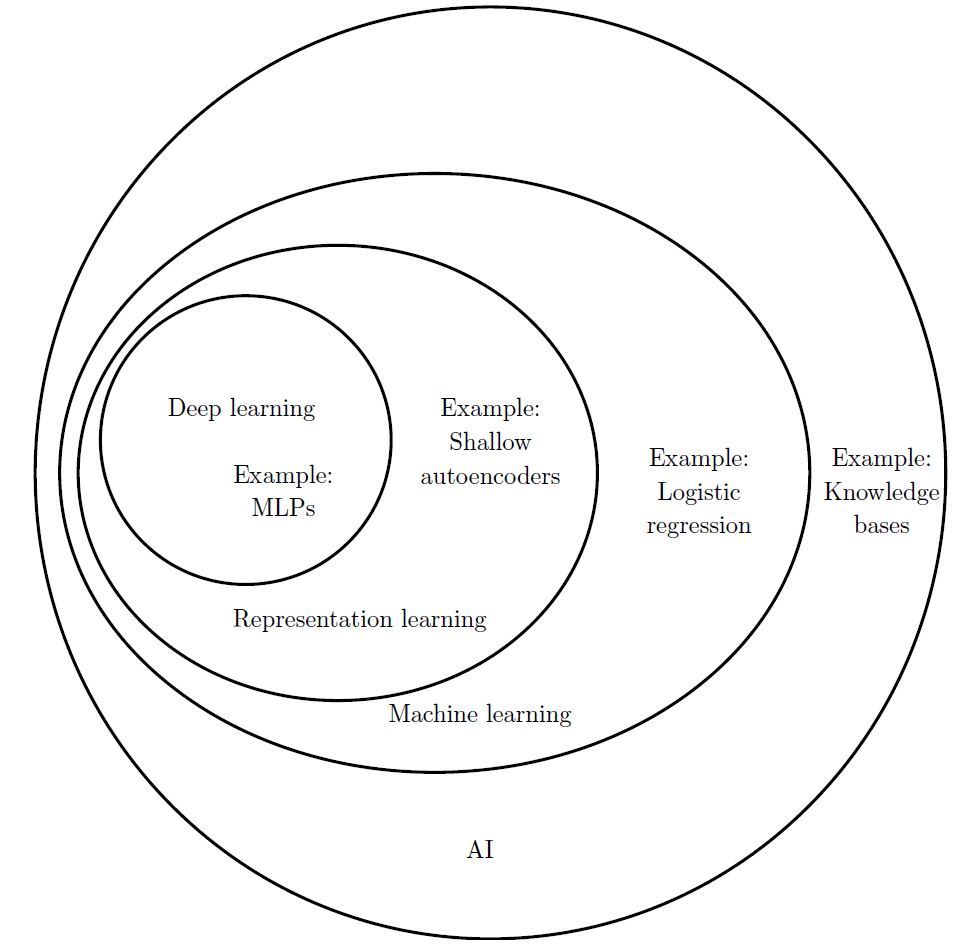
\includegraphics[width=0.7\linewidth]{DL diagram.png}
    \captionsetup{format=hang}
    \caption{Diagram Venna ukazujący zależności pomiędzy głębokim uczeniem, uczeniem reprezentacji, uczeniem maszynowym a~sztuczną inteligencją \cite{goodfellow}}
    \label{fig:diagram1}
\end{figure}

Głębokie uczenie jest implementowane przy pomocy głębokich sieci neuronowych (ang. \emph{deep neural networks}), których architektura opiera się na połączonych ze sobą neuronach. Każde połączenie pomiędzy neuronami jest reprezentowane przy pomocy wagi, która wskazuje jak ważna jest wartość danego neuronu (w~konkretnym połączeniu z~innym neuronem) z~perspektywy całej sieci. Neurony są grupowane w~warstwy (w~liczbie zazwyczaj od kilku do nawet kilkuset), a~te z~kolei grupuje się w~bloki, czyli funkcjonalne jednostki przetwarzania danych. Głębokie sieci neuronowe są implementowane przy pomocy bardzo zróżnicowanych architektur jednak architektury te zazwyczaj składają się z~kilku podstawowych elementów (warstw). Do najważniejszych z~nich należą: warstwa konwolucyjna, warstwa liniowa, warstwa grupująca, warstwa aktywacji, warstwa \emph{dropout} oraz warstwa normalizacji partiami. Najbardziej popularnymi klasami głębokich sieci neuronowych są konwolucyjne sieci neuronowe (ang. \emph{convolutional neural networks}) oraz rekurencyjne sieci neuronowe (ang. \emph{recurrent neural networks}). Konwolucyjne sieci neuronowe charakteryzują się tym, iż ich architektura jest oparta o~warstwy splotowe, które pozwalają na efektywną ekstrakcję cech. Natomiast rekurencyjne sieci neuronowe charakteryzuje występowaniem cyklicznych połączeń pomiędzy neuronami, które umożliwiają analizę danych o~charakterze sekwencyjnym. 

\paragraph*{Warstwa konwolucyjna (splotowa)}

Warstwa konwolucyjna (ang. \emph{convolution layer}) jest podstawową jednostką przetwarzania w~głębokich sieciach neuronowych. Składa się ona z~szeregu filtrów (ang. \emph{filter} / \emph{kernel}), o~rozmiarach zazwyczaj nieprzekraczających kilku pikseli, które przesuwając się po danych wejściowych, reprezentowanych zazwyczaj w~formie wielowymiarowej macierzy, wykonują operację iloczynu Hadamarda, po którym następuje sumowanie wszystkich elementów uzyskanej macierzy do pojedynczych liczb (ekstrakcja cech). Liczby te następnie tworzą nową macierz, która jest nazywana mapą cech (ang. \emph{features map}). Każdy z~filtrów zastosowanych w~warstwie konwolucyjnej składa się początkowo z~losowych wartości, w~trakcie trenowania sieci, w~kolejnych iteracjach obliczeń (zwanych powszechnie epokami (ang. \emph{epochs})), następuje aktualizacja wartości filtrów, aby sieć nabierała pożądanych od niej własności. Każdy filtr warstwy splotowej tworzy własną mapę cech, więc deklarując liczbę filtrów w~danej warstwie, deklarujemy ile map cech (unikalnych atrybutów danego zbioru danych) na wyjściu z danej warstwy chcemy uzyskać. W~ramach warstwy konwolucyjnej, poza rozmiarem filtrów (ich kształtem), należy zdefiniować jeszcze kilka ważnych parametrów (hiperparametrów\footnote{Hiperparametrami sieci neuronowej nazywamy najważniejsze parametry tej sieci, które są definiowane przez jej architekta przed przystąpieniem do procesu trenowania.}), takich jak: 
\begin{itemize}
\item krok (ang. \emph{stride}) o~jaki filtr będzie przesuwany w~czasie ekstrakcji cech,
\item \emph{padding} czyli wskazanie czy chcemy by tworzone mapy cech utrzymały rozdzielczość danych wejściowych, jeśli tak to jakimi wartościami należy uzupełnić ewentualne braki powstałe na skutek różnic pomiędzy rozmiarem danych wejściowych a~rozmiarem filtra (domyślnie braki są uzupełniane wartością zero),
\item dylacja (ang. \emph{dilation}) czyli odległość pomiędzy punktami filtra - domyślnie filtr jest nakładany na sąsiadujące ze sobą elementy macierzy wejściowej, ale można przy pomocy dylacji ustawić by był on nakładany na przykład na co drugi jej element (dylacja równa 2).
\end{itemize}

Szczególnym przypadkiem warstwy konwolucyjnej jest \textbf{konwolucja transponowana} (ang. \emph{transposed convolution}), którą można określić jako operację odwrotną do operacji splotu. O~ile celem konwolucji jest uzyskanie uproszczonej reprezentacji danych wejściowych, o tyle konwolucja transponowana stara się przetransformować dane wejściowe o~mniejszej wymiarowości,, do danych o~większym wymiarze. Stąd też konwolucję transponowaną często określa się jako nadpróbkowanie (ang. \emph{upsampling}) i~jest ona najczęściej wykorzystywana przy zadaniach związanych z rekonstrukcją danych. Innym szczególnym przypadkiem warstwy konwolucyjnej jest \textbf{konwolucja z~filtrem o rozmiarze 1x1}, której najczęstszym zadaniem jest redukcja liczby map cech w~danym miejscu sieci neuronowej, dzięki czemu dochodzi do istotnego zmniejszenie rozmiaru tej sieci bez dużego uszczerbku dla jej efektywności. 

\paragraph*{Warstwa liniowa}

Warstwa liniowa (ang. \emph{linear layer} / \emph{dense layer} / \emph{fully-connected layer}) to najprostsza ze wszystkich warstw stosowanych w~głębokich sieciach neuronowych. Jej zadaniem jest zastosowanie transformacji liniowej na danych pochodzących z~poprzedzającej ją warstwy. Hiperparametrami warstwy liniowej są: liczba wejść (ang. \emph{input size}), liczba wyjść (ang. \emph{output size}) oraz flaga wskazująca czy przy przeprowadzaniu transformacji linowej należy stosować przesunięcie (ang. \emph{bias}).

\paragraph*{Warstwa grupująca}

Warstwa grupująca (ang. \emph{pooling layer}) to jednostka, której zadaniem jest redukcja wymiarowości danych wejściowych poprzez zastosowanie wybranej funkcji grupującej (najczęściej funkcji maximum lub funkcji średniej). Podobnie jak w przypadku warstwy splotowej, po danych wejściowych warstwy grupującej przesuwany jest filtr o~wymiarach kilku pikseli, którego zadaniem jest wybranie największej wartości z~danego zakresu danych (\emph{max pooling}) lub wyliczenie średniej dla tego zakresu (\emph{average pooling}). W~ten sposób, dla filtra (okna) warstwy grupującej o~wymiarach na przykład 2x2, cztery wartości danych wejściowych są redukowane do jednej wartości - maksimum lub średniej z~nich. W~ramach warstwy grupującej definiowany jest taki sam zbiór hiperparametrów jak w~przypadku warstwy konwolucyjnej czyli: rozmiar filtra, krok filtra, \emph{padding} oraz~dylacja - mają one dokładnie takie samo zastosowanie jak w~przypadku warstwy splotowej. Poza zdefiniowanymi powyżej podstawowymi operacjami grupującymi często wyróżnia się jeszcze operację globalnego grupowania do maksimum (ang. \emph{global max pooling}) oraz operację globalnego grupowania do średniej (ang. \emph{global average pooling}), które polegają na zastosowaniu funkcji maksimum / średniej nie na poziomie filtrów, ale na poziomie całych kanałów danych wejściowych. 

\paragraph*{Warstwa aktywacji}

Warstwa aktywacji (ang. \emph{activation function}) przetwarza dane pochodzące z~map cech wygenerowanych w~poprzednich warstwach po to by nadać im niezbędną nieliniowość. Jest ona konieczna po to by sieci neuronowe były w~stanie nauczyć się skomplikowanych wzorców występujących w~analizowanych przez nie danych. Do najpopularniejszych warstw (funkcji) aktywacji wykorzystywanych w~głębokich sieciach neuronowych można zaliczyć:

\begin{itemize}
\item \emph{sigmoid}:
 \begin{equation}
simg(x) = \frac{1}{1 + e^{-x}}
\end{equation}
\item \emph{tangens hiperboliczny}: 
 \begin{equation}
tanh(x) = \frac{e^x-e^{-x}}{e^{x}+e^{-x}}
\end{equation}
\item \emph{ReLU}:
 \begin{equation}
 ReLU(x) = max(x, 0)
\end{equation}
\item \emph{Leaky ReLU}:
 \begin{equation}
  LReLU(x) = 
 \begin{cases}
  x & \text{dla x > 0}  \\
  0,01 \cdot x & \text{dla x $\leq$ 0} \\
  \end{cases}
\end{equation}
\item \emph{Parametric ReLU}:
 \begin{equation}
 PReLU(x) =  
 \begin{cases}
  x & \text{dla x > 0}  \\
  \alpha \cdot x & \text{dla x $\leq$ 0} \\
  \end{cases}
\end{equation}
\item \emph{Exponential Linear Unit}:
 \begin{equation}
 ELU(x) = 
  \begin{cases}
  x & \text{dla x >  0}  \\
  \alpha \cdot (e^{x}-1)  & \text{dla x $\leq$ 0} \\
  \end{cases}
\end{equation}
\item \emph{softmax\footnote{Softmax jest specyficzną funkcją aktywacji, gdyż jej głównym zadaniem jest normalizacja danych wyjściowych sieci neuronowej do rozkładu prawdopodobieństwa}}:
 \begin{equation}
 softmax(x_i) = \frac{e^{x_i}}{\sum_{j=1}^{n}e^{x_j}}
\end{equation}
\end{itemize}

Funkcje \emph{sigmoid} oraz \emph{tangens hiperboliczny}, ze względu na swoją złożoność obliczeniową i~fakt, iż mogą się przyczyniać do występowania problemu zanikającego gradientu, są stosunkowo rzadko wykorzystywane w~bieżących architekturach głębokich sieci neuronowych. Najczęściej stosowaną funkcją aktywacji jest \emph{ReLU}, głównie ze względu na swoją prostotę i~skuteczność. Często zarzuca się jej jednak brak różniczkowalności w~punkcie 0 oraz zerową wartość pochodnej dla ujemnych argumentów, która może powodować wymieranie neuronów (\emph{dead ReLU}). Stąd też opracowane zostały różne modyfikacje funkcji ReLU, które starają się rozwiązać te problemy przy okazji zachowując wszystkie najważniejsze zalety tej funkcji aktywacji (\emph{Leaky ReLU}, \emph{Parametric ReLU}, \emph{Exponential Linear Unit}).

\paragraph*{Warstwa \emph{dropout}}

Głębokie sieci neuronowe ze względu na ogromną liczbę trenowalnych parametrów (wag) są szczególnie podatne na problem zwany przeuczeniem (ang. \emph{overfitting}), który polega na zbyt dokładnym dopasowaniu się sieci neuronowej do konkretnych danych uczących, przez co sieć ta staje się mniej skuteczna w~generowaniu prawidłowych predykcji dla danych z~poza zbioru uczącego (rośniej jej błąd generalizacji). Zadaniem warstwy \emph{dropout} jest zmiana funkcjonowania sieci neuronowej w~taki sposób by jak najbardziej zminimalizować błąd generalizacji modelu. Rozwiązaniem tego problemu, uzyskiwanym w~ramach warstwy \emph{dropout}, jest losowe wyłączanie (zerowanie aktywacji) niektórych neuronów sieci w~każdej epoce jej uczenia, po to by miała ona zdolność wyłapywania jak najbardziej uniwersalnych cech danego zbioru danych, niezwiązanych z~konkretnymi wartościami poszczególnych neuronów. To jaki procent wszystkich neuronów zostanie wyłączonych w~konkretnej epoce jest definiowane przy pomocy hiperparametru \emph{p}, czyli prawdopodobieństwa, że dany neuron zostanie wyzerowany. 

Warstwę \emph{dropout} w~związku z~jej właściwością zapobiegania przeuczeniu sieci neuronowej nazywa się często techniką regularyzacji. Inną równie często stosowaną techniką regularyzacji modelu jest \textbf{augmentacja danych} (ang. \emph{data augmentation}), czyli technika transformacji danych treningowych sieci neuronowej w~taki sposób by jak najbardziej je zróżnicować, uzyskując tym samym większą liczbę przypadków uczących. Jednymi z~najpopularniejszych sposobów przekształcania danych uczących są: skalowanie (ang. \emph{scale}), przesuwanie (ang. \emph{shift}), losowe obracanie (ang. \emph{random rotation}), losowe wycinanie fragmentów (ang. \emph{random crop}) czy normalizacja (ang. \emph{normalization}). 

\paragraph*{Warstwa normalizacji partiami}

Zadaniem warstwy normalizacji partiami (ang. \emph{batch normalization layer}) jest zaradzenie problemowi ciągłej zmiany rozkładów wartości generowanych przez poszczególne warstwy głębokich sieci neuronowych wraz z~postępem ich uczenia. W~związku z~tym zjawiskiem poszczególne warstwy modelu dużą część swojej pracy poświęcają na dostosowanie się do wewnętrznego przesunięcia rozkładów (ang. \emph{internal covariate shift}), zamiast spożytkować tę pracę na efektywną naukę. Rozwiązaniem tego problemu było dodanie nowej warstwy do architektury modelu, której zadaniem była odpowiednia standaryzacja wartości wyjściowych z~poprzedniej warstwy poprzez odjęcie średniej wartości w~danej partii (ang. \emph{batch}) i~podzielenie przez odchylenie standardowe z~tej partii. Zastosowanie warstwy normalizacji partiami pozwala na efektywniejszą naukę sieci neuronowej - sieć w~czasie treningu szybciej minimalizuje funkcję strat.

\subsection{Ewolucja architektur głębokiego uczenia}

Termin głębokie uczenie zyskał w~ostatnim czasie ogromną popularność, głównie dzięki mnogości zastosowań jaką ta gałąź sztucznej inteligencji znalazła w~szerokiej gamie dziedzin życia codziennego - od samochodów autonomicznych, przez asystentki głosowe w~urządzeniach mobilnych / \emph{smart home}, aż po systemy rozpoznawania twarzy na lotniskach. Jednak termin ten nie jest nowy w~świecie nauki, był on używany przez naukowców od wielu lat, a~jego korzenie można datować na lata 40-ste dwudziestego wieku. 

\subsubsection{Cybernetyka (1943 - 1969)}
Praprzodkiem głębokiego uczenia, rozwijanym w~latach 40., 50. i~60. XX wieku, była cybernetyka, czyli nauka badająca mechanizmy kontroli i~komunikacji u~zwierząt i~maszyn \cite{wiener}. W~ramach cybernetyki naukowcy starali się stworzyć modele mogące naśladować biologiczną pracę mózgu. Najważniejszymi osiągnięciami tamtego okresy były następujące modele liniowe:

\begin{itemize}
\item \textbf{model neuronu} stworzony w~1943 roku przez Warrena McCullocha i~Waltera Pittsa (przez autorów nazywany \emph{Threshold Logic Unit}) \cite{mcculloch}, który oparty był na równaniu liniowym z~arbitralnie dobranymi wagami przy zmiennych wejściowych (patrz rysunek \ref{fig:neuron1}),

\begin{figure}[!h]
    \centering 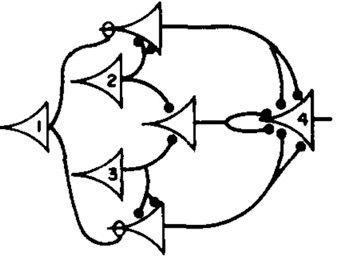
\includegraphics[width=0.6\linewidth]{Neuron.jpeg}
    \captionsetup{format=hang}
    \caption{Przykładowy schemat neuronu zaprezentowany w~1943 roku przez Warrena McCullocha i~Waltera Pittsa \cite{mcculloch}}
    \label{fig:neuron1}
\end{figure}

\item \textbf{model perceptronu} zaprezentowany w~1958 roku przez Franka Rosenblatta \cite{rosenblatt}, który był rozwinięciem neuronu o~możliwość samodzielnej nauki wartości wag przy poszczególnych zmiennych na podstawie danych treningowych\footnote{Wielu naukowców uznaje model perceptronu zaprezentowany przez Franka Rosenblatta za pierwszą współczesną sieć neuronową (\emph{feedforward neural network}).} (patrz rysunek \ref{fig:perceptron1}),

\begin{figure}[!h]
    \centering 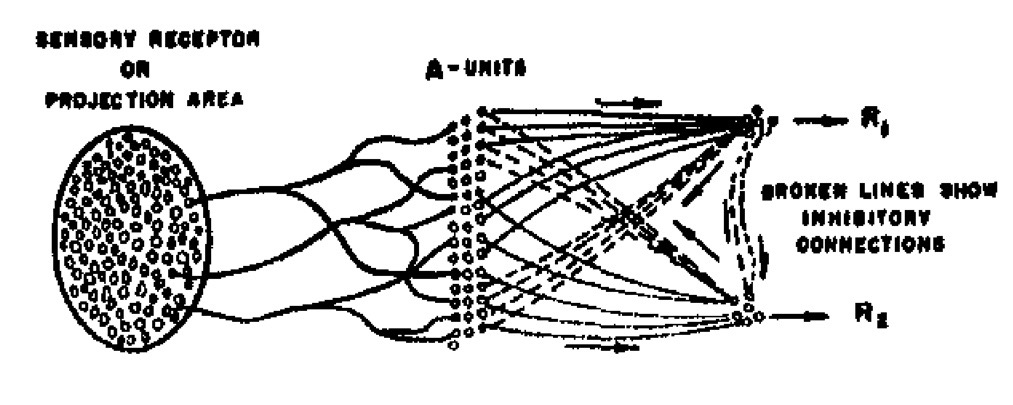
\includegraphics[width=1.0\linewidth]{Perceptron.jpeg}
    \captionsetup{format=hang}
     \caption{Schematyczna reprezentacja połączeń w~prostym perceptronie zaprezentowana w~1958 roku przez Franka Rosenblatta \cite{rosenblatt}}
    \label{fig:perceptron1}
\end{figure}

\item model adaptacyjnego neuronu liniowego stworzony przez Bernarda Widrowa i~Teda Hoffa, określany skrótem \textbf{ADALINE} (ang. \emph{Adaptive Linear Neuron}), który od perceptronu różnił się między innymi tym, że w~czasie uczenia jego wagi były dostosowywane do ważonej sumy wartości wejściowych (patrz rysunek \ref{fig:adaline1}).
\end{itemize} 

\vspace{1cm}

\begin{figure}[!h]
    \centering 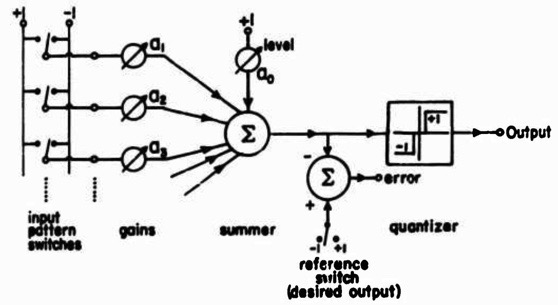
\includegraphics[width=0.8\linewidth]{ADALINE.jpeg}
    \captionsetup{format=hang}
      \caption{Schemat ADALINE zaprezentowany w 1960 roku przez Bernarda Widrowa i~Teda Hoffa \cite{widrow}}
    \label{fig:adaline1}
\end{figure}

Pod koniec lat 60. XX wieku popularność modeli tworzonych w~nurcie cybernetyki istotnie zmalała za sprawą licznych ograniczeń modeli liniowych wskazywanych przez część naukowców. W~1969 roku ukazała się słynna książka Marvina Minsky'ego i~Seymoura Paperta pod tytułem \emph{Perceptrons: an introduction to computational geometry} \cite{minsky}, która wskazywała na liczne ograniczenia modelu pojedynczego perceptronu Rosenblatta, takie jak na przykład fakt, iż nie jest on w~stanie nauczyć się prostej operacji logicznej \emph{XOR} (ani żadnej innej operacji nieseparowalnej liniowo). Minksy i~Papert wskazywali jednocześnie, iż takich operacji mogłaby nauczyć się sieć złożona z~kilku perceptronów, lecz nie ma efektywnych sposobów uczenia takich sieci. Ta publikacja istotnie przyczyniła się do spadku popularności modeli uczenia inspirowanych biologicznie. 

\subsubsection{Konekcjonizm (1980 - 1998)}

Kolejnym przodkiem głębokiego uczenia, który najdynamiczniej rozwijał się  w~latach 80. i~90. XX wieku, był konekcjonizm, czyli podejście z~dziedziny kognitywistyki, które miało za zadanie wyjaśnić zjawiska umysłowe przy pomocy modeli neuronowych. Główną ideą tego nurtu sztucznej inteligencji było przekonanie, iż duża liczba prostych jednostek obliczeniowych połączonych w~sieć może umożliwić uzyskanie inteligentnego zachowania u~maszyny. 

\paragraph*{Neocognitron}

Jednymi z~najważniejszych artykułów początkowej fazy konekcjonizmu były artykuły Kunihiko Fukushimy wprowadzające pojęcia \textbf{\emph{cognitronu}} \cite{fukushima1} i~\textbf{\emph{neocognitronu}} \cite{fukushima2}, czyli samoorganizującej się sieci neuronowej (wzorowanej na systemie widzenia ssaków), która jest w~stanie rozpoznawać wzorce według geometrycznego podobieństwa ich kształtu. \emph{Neocognitron} był rozwinięciem \emph{cognitronu} wprowadzającym do sieci neuronowej charakter splotowy, co pozwoliło na uniezależnienie odpowiedzi modelu od umiejscowienia wzorca.  

\begin{figure}[!h]
    \centering 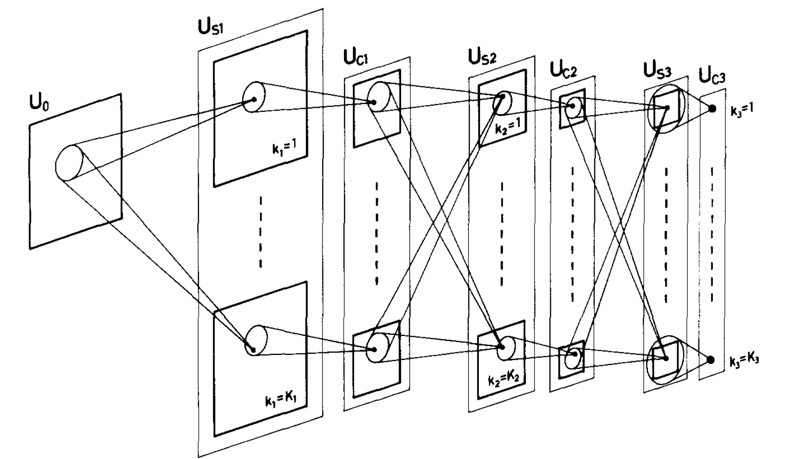
\includegraphics[width=0.9\linewidth]{Neocognitron.jpeg}
    \captionsetup{format=hang}
    \caption{Diagram pokazujący połączenia pomiędzy warstwami w~neocognitronie zaprezentowanym w~1980 roku przez Kunihiko Fukushimę \cite{fukushima2}}
    \label{fig:neocognitron1}
\end{figure}

\emph{Neocognitron} można więc uznać za jeden z~pierwszych modeli z~dziedziny \textbf{konwolucyjnych sieci neuronowych}. Składał się on z~sześciu warstw splotowych przeplatanych warstwami grupującymi (patrz rysunek \ref{fig:neocognitron1}). Wejściem do modelu \textit{neocognitronu} były obrazy o rozmiarach 16~x~16, a~każda warstwa splotowa zawierała 24 filtry o~wymiarach 5~x~5. Po wytrenowaniu model Fukushimy był w~stanie rozpoznać pięć cyfr („0”, „1”, „2”, „3”, „4”) i~cztery litery („X”, „Y”, „T”, „Z”).

\paragraph*{Recurrent Neural Network (RNN)}

Prace Fukushimy przyczyniły się do rozwoju konwolucyjnych sieci neuronowych, które dawały bardzo obiecujące wyniki w~dziedzinie analizy obrazu, jednak miały one ograniczony potencjał zastosowania w~dziedzinach, w~których liczy się analiza całych sekwencji danych, jak na przykład analiza mowy, dźwięku, wideo czy pisma odręcznego. Do tego typu zastosowań potrzebna jest sieć, która dysponuje wewnętrzną pamięcią, po to by móc wyłapywać zależności nie tylko wewnątrz bieżącego fragmentu danych, ale także pomiędzy kolejnymi pojawiającymi się sekwencjami. Głębokie sieci neuronowe, które posiadają taką własność, nazywamy \textbf{rekurencyjnymi sieciami neuronowymi}. Jednym z~pierwszych artykułów z nurtu konekcjonizmu, wprowadzających rekurencyjne połączenia do sieci neuronowych, i~w~ten sposób tworzących sieci z dynamiczną pamięcią, był artykuł \emph{Serial order: A parallel distributed processing approach} napisany w~1986~roku przez Michaela Irwina Jordana \cite{jordan}. 

\begin{figure}[!h]
    \centering 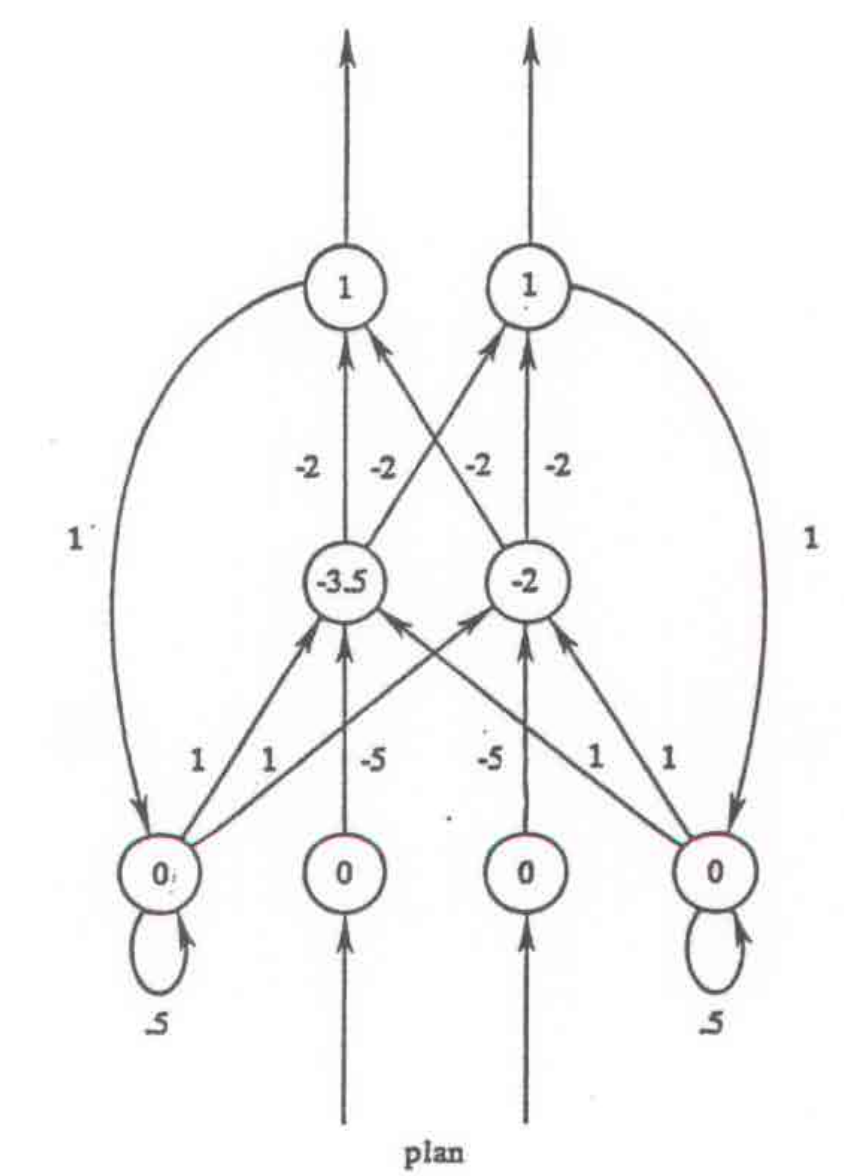
\includegraphics[width=0.3\linewidth]{Jordan.png}
    \captionsetup{format=hang}
    \caption{Diagram pokazujący połączenia w~sieci rekurencyjnej zaprezentowanej w~1986 roku przez Michaela Irwina Jordana \cite{jordan}}
    \label{fig:jordan1}
\end{figure}

W~swoim artykule Jordan proponuje nowatorskie podejście, które umożliwia nauczenia się sekwencji zdarzeń przez sieć neuronową, gdzie każda ukryta komórka (ang. \emph{hidden cell}) otrzymuje swoje własne dane wyjściowe z~odpowiednim, ustalonym opóźnieniem (patrz rysunek \ref{fig:jordan1}).

\paragraph*{Backpropagation}

Dynamiczny rozwój konekcjonizmu nie byłby możliwy bez opracowania efektywnego \textbf{algorytmu wstecznej propagacji błędu} (ang. \emph{backpropagation algorithm}). Jako jego twórcę uznaje się Paula Werbosa, który opisał go już w~1974 roku w~swojej rozprawie doktorskiej. Jednak algorytm ten nie zyskał dużego rozgłosu aż do 1986~roku, kiedy to David Rumelhart, Geoffrey Hinton i~Ronald Williams w~swoim artykule \emph{Learning representations by back-propagating errors} \cite{rumelhart} pokazali zastosowanie algorytmu wstecznej propagacji błędu do trenowania \textbf{wielowarstwowego perceptronu} (ang. \emph{Multilayer Perceptron}).

\begin{figure}[!h]
    \centering 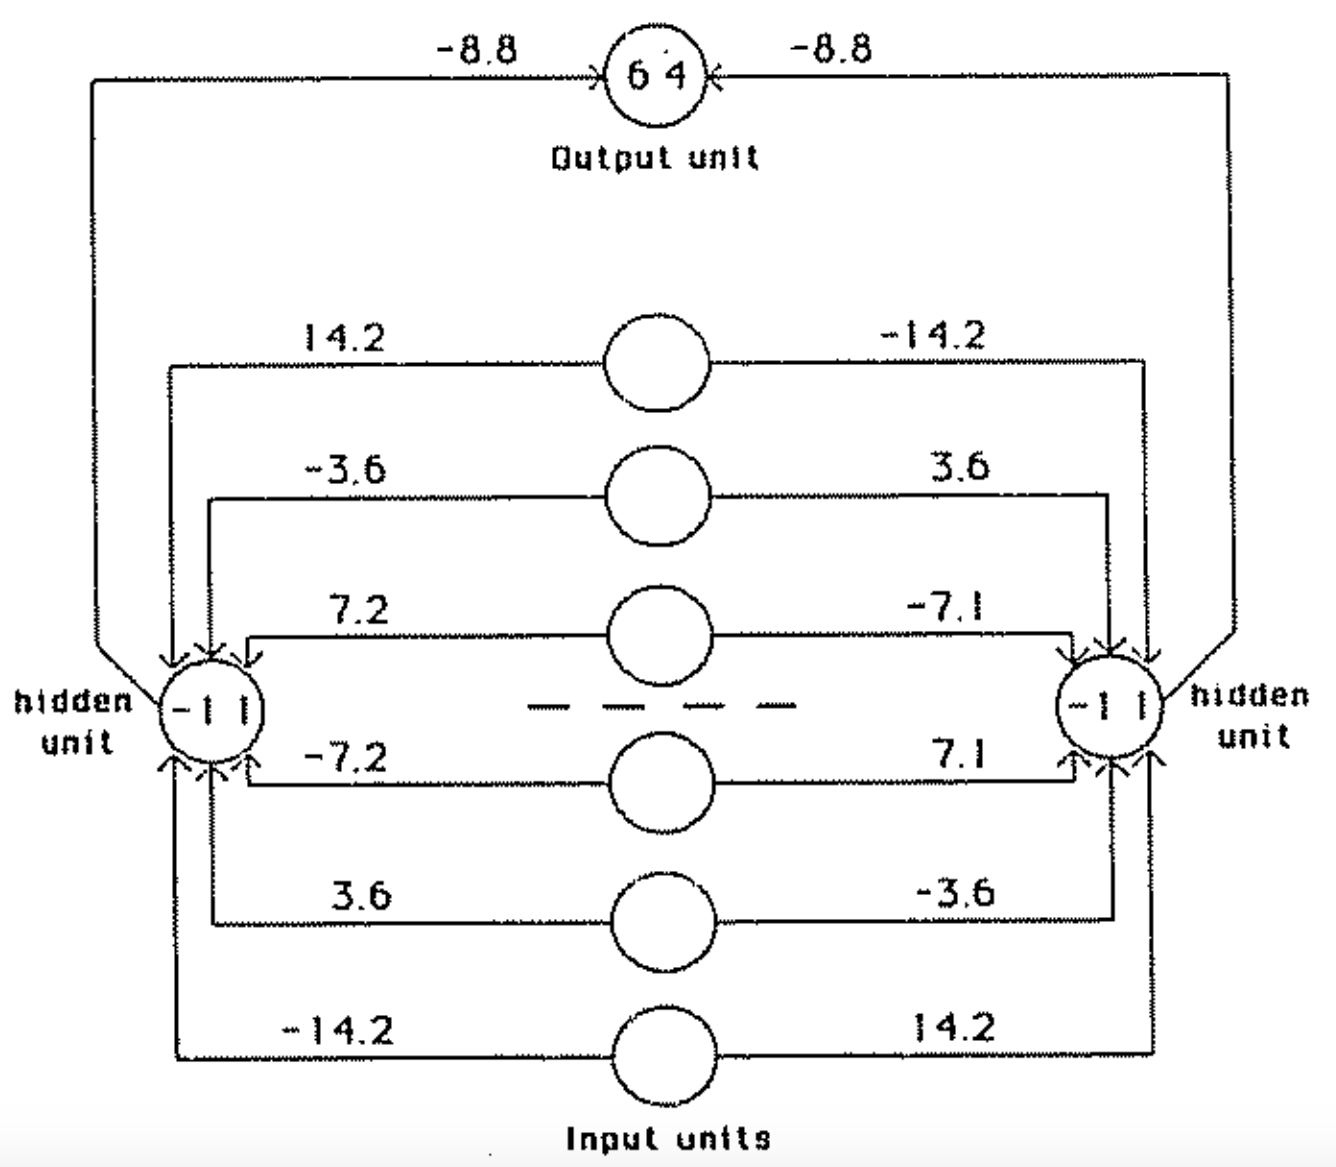
\includegraphics[width=0.4\linewidth]{MLP.png}
    \captionsetup{format=hang}
      \caption{Schemat wielowarstwowego perceptronu zaprezentowany w 1986 roku przez Davida Rumelharta, Geoffreya Hintona i~Ronalda Williamsa \cite{rumelhart}}
    \label{fig:mlp1}
\end{figure}

 W~czasie treningu sieci neuronowej algorytm wstecznej propagacji błędu wylicza gradient funkcji strat w~odniesieniu do wag tej sieci przy pomocy reguły łańcuchowej (ang. \emph{chain rule}). Gradient ten jest wyliczany dla każdej warstwy sieci neuronowej poczynając od najgłębszych warstw przechodząc iteracyjnie ku warstwom początkowym. 


\paragraph*{LeNet-5}

Kontynuatorem koncepcji Kunihiko Fukushimy, który do wytrenowania splotowej sieci neuronowej o~architekturze wzorowanej na \emph{neocognitronie} zastosował algorytm wstecznej propagacji błędu przedstawiony przez Davida Rumelharta, Geoffreya Hintona i~Ronalda Williamsa, był francuski naukowiec Yann André LeCun. W~swoich dwóch artykułach \emph{Backpropagation Applied to Handwritten Zip Code Recognition} z~1989 roku \cite{lecun1} i~\emph{Gradient-based learning applied to document recognition} z~1998 roku \cite{lecun2} zaprezentował on konwolucyjną sieć neuronową, która była w~stanie z~zadowalającą, jak na tamten czas, skutecznością rozpoznawać znaki pisma odręcznego. Sieć z~1998 roku zyskała nazwę \textbf{\emph{LeNet-5}}, składała się z~około 60 tysięcy trenowalnych parametrów podzielonych na siedem warstw (cztery splotowo-grupujące i~trzy warstwy gęste) o~filtrach w~rozmiarze 5~x~5, a~jako wejście przyjmowała obrazy o~rozdzielczości 32~x~32~(patrz rysunek \ref{fig:lenet1}). Co ciekawe, żeby ograniczyć liczbę trenowanych parametrów / połączeń niektóre warstwy modelu LeCunna łączyły się jedynie z~wybranymi filtrami z~warstw poprzednich. 

\begin{figure}[!h]
    \centering 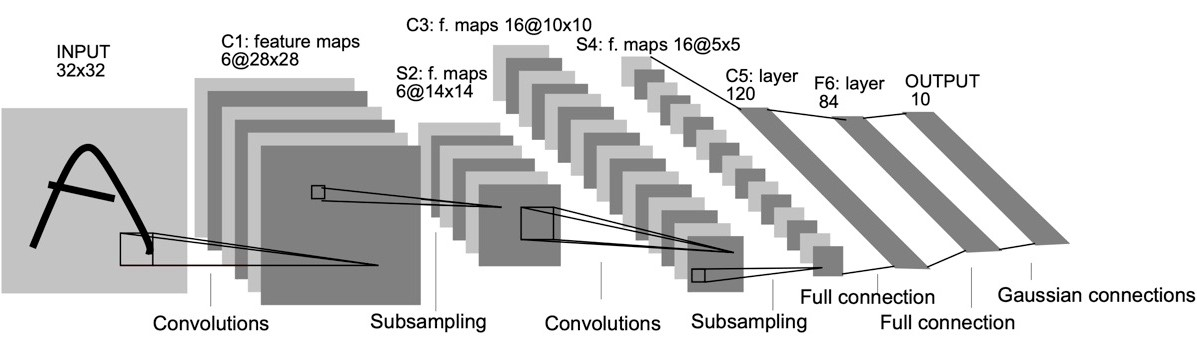
\includegraphics[width=1.0\linewidth]{LeNet-5.jpeg}
    \captionsetup{format=hang}
    \caption{Architektura sieci \emph{LeNet-5} stworzona w~1998 roku przez Yanna LeCuna \cite{lecun2}}
    \label{fig:lenet1}
\end{figure}

Sieć \emph{LeNet-5} stała się kamieniem milowym w~rozwoju sieci neuronowych, w~szczególności konwolucyjnych sieci neuronowych, gdyż pokazała, iż wielowarstwowe modele mogą osiągać w~niektórych zastosowaniach lepsze rezultaty niż inne dostępne w~tamtym czasie techniki rozpoznawania pisma odręcznego. Artykuł Yanna LeCunna z~1998 roku przyczynił się również do powstania sprawdzonego schematu trenowania sieci neuronowej z~warstwami splotowo-grupującymi zakończonymi warstwami gęstymi, schemat ten w~kolejnych latach był wielokrotnie powielany i~rozszerzany przez wielu autorów, lecz zasadniczy trzon architektury splotowych sieci neuronowych pozostał praktycznie niezmieniony.

\paragraph*{Long Short-Term Memory (LSTM)}

Drugim kluczowym artykułem, który powstał u~schyłku konekcjonizmu był artykuł z~1997 roku zatytułowany \emph{Long short-term memory} napisany przez Seppa Hochreitera i~Jürgena Schmidhubera \cite{hochreiter}. Wprowadzał on nową architekturę \textbf{\emph{LSTM}} w~dziedzinie rekurencyjnych sieci neuronowych, która pozwalała rozwiązać istotny problem dotykający w~tamtym czasie sieci \emph{RNN}, a~mianowicie problem zanikającego gradientu (ang. \emph{vanishing gradient problem})\footnote{Problem zanikającego gradientu pojawia się gdy, po przekroczeniu pewnej głębokości (długości przetwarzanej sekwencji), sieci neuronowe nie są w~stanie efektywnie uczyć się (aktualizować swoich wag), gdyż gradient błędów dla głębokich warstw (odległych sekwencji) staje się zbyt mały.}. Sieć \emph{LSTM} wprowadzała wewnętrzne mechanizmy zwane bramkami (ang. \emph{gates}), które pozwalały kontrolować przepływ informacji przetwarzanych przez sieć neuronową. Bramki te razem z~komórkami pamięci (ang. \emph{memory cells}) miały za zadanie nauczyć się, które informacje z~poprzednich sekwencji danych należy zatrzymać (uznając je za ważne), a~które można pominąć (nieważne). W~ramach modelu \emph{LSTM} wyróżniano trzy bramki:

\begin{itemize}
\item bramkę zapomnienia (ang. \emph{forget gate}) - bramka ta decydowała, którą informację należy zapomnieć, a którą zachować,
\item bramkę wejścia (ang. \emph{input gate}) - bramka ta aktualizowała wewnętrzny stan komórki pamięci,
\item bramkę wyjścia (ang. \emph{output gate}) - bramka ta decydowała jaki powinien być następny ukryty stan (ang. \emph{hidden state}) sieci. 
\end{itemize}

\begin{figure}[!h]
    \centering 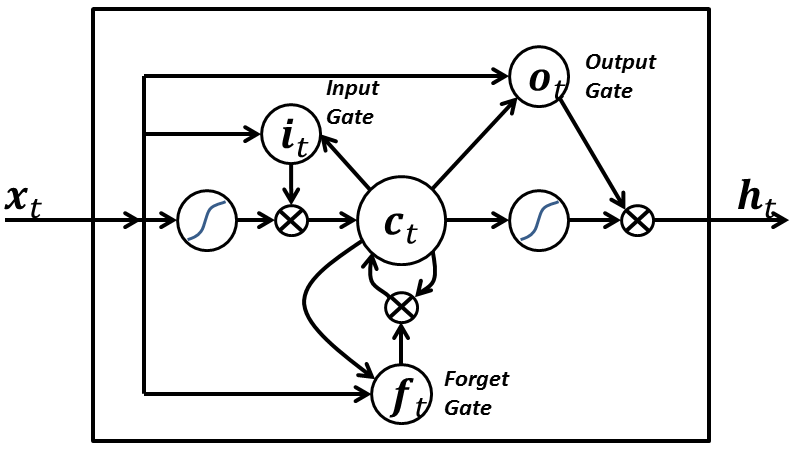
\includegraphics[width=0.9\linewidth]{LSTM.png}
    \captionsetup{format=hang}
    \caption{Architektura sieci \emph{LSTM} zaprezentowanej w~1997 roku przez Seppa Hochreitera i~Jürgena Schmidhubera \cite{hochreiter}}
    \label{fig:lstm1}
\end{figure}

Istotnymi ograniczeniami rozwoju sieci neuronowych tworzonych u~schyłku XX wieku były skromne, z~dzisiejszej perspektywy, zasoby obliczeniowe ówczesnych komputerów, które powodowały, iż wytrenowanie nawet najprostszej sieci neuronowej trwało wiele dni, stąd też metody stosowane przez przedstawicieli nurtu konektywizmu stopniowo traciły na popularności. 

\subsubsection{Głębokie uczenie (2006 - 2020)}

Za swoisty renesans nurtu konektywizmu i~właściwy początek głębokiego uczenia, można uznać rok 2006 kiedy to Hinton G., Osindero S. i Teh Y. W. w~swoim artykule \emph{A~Fast Learning Algorithm for Deep Belief Nets} \cite{hinton} pokazali, że sieci głębokiej wiarygodności mogą być efektywnie trenowane przy pomocy strategii o~nazwie chciwe warstwowe trenowanie wstępne (ang. \emph{greedy layer-wise pretraining}), która pozwalała zmniejszyć problem zanikającego gradientu oraz wzmocnić generalizację na zbiorze testowym poprzez efektywniejszą inicjalizację wag. Kolejni autorzy, wzorując się na pracy zespołu Geoffreya Hintona, szybko pokazali, że strategia chciwego warstwowego trenowania wstępnego może być zastosowana też do innych rodzajów głębokich sieci neuronowych, co otworzyło drogę do tworzenia modeli o~niedostępnych dotąd głębokościach.

\paragraph*{AlexNet}

W~tym samym czasie, dynamiczny rozwój przemysłu gier komputerowych i~związany z~nim rozwój kart graficznych, umożliwił bezprecedensowy wzrost efektywności trenowania głębokich sieci neuronowych - zamiast tradycyjnego trenowania sieci na jednostkach CPU (ang. \emph{central processing unit}) zaczęto je trenować na jednostkach GPU (ang. \emph{graphics processing unit}). Przełomowym artykułem w~zakresie trenowania modelu na wielu kartach graficznych był artykuł \emph{ImageNet classification with deep convolutional neural networks} opublikowany w~2012 roku przez Krizhevsky A., Sutskever I.  i~Hinton G. \cite{alexnet}. Co prawda nie był to pierwszy artykuł ukazujący ogromne możliwości GPU w~zakresie trenowania głębokich sieci neuronowych\footnote{Pierwszym takim artykułem był \emph{High Performance Convolutional Neural Networks for Document Processing} napisany w~2006 roku przez Chellapilla K., Puri S. i~Simard P.}, jednak stał się jednym z~najczęściej cytowanych artykułów w~dziedzinie głębokiego uczenia, gdyż łączył w~sobie wiele innowacyjnych na tamten czas rozwiązań takich jak:

\begin{itemize}
\item trening sieci na ogromnym zbiorze danych - \emph{ImageNet} z~15 milionami podpisanych obrazów dla ponad 22 tysięcy kategorii,
\item architektura modelu w~postaci konwolucyjnej sieci neuronowej, 
\item trening sieci neuronowej jednocześnie na dwóch kartach graficznych,
\item \emph{ReLU} jako funkcja aktywacji przyspieszająca zbieżność procesu uczenia, 
\item augmentacja danych treningowych realizowana poprzez translację, obroty horyzontalne i~wycinanie fragmentów obrazów, 
\item zastosowanie warstw \emph{dropout} w~celu zapobiegnięcia przetrenowaniu sieci,
\item trenowanie modelu w~pakietach przy użyciu stochastycznego spadku gradientu (ang. \emph{batch stochastic gradient descent}) z~jasno określonymi parametrami momentum i~spadku wagi (ang. \emph{weight decay}).
\end{itemize}

\begin{figure}[!h]
    \centering 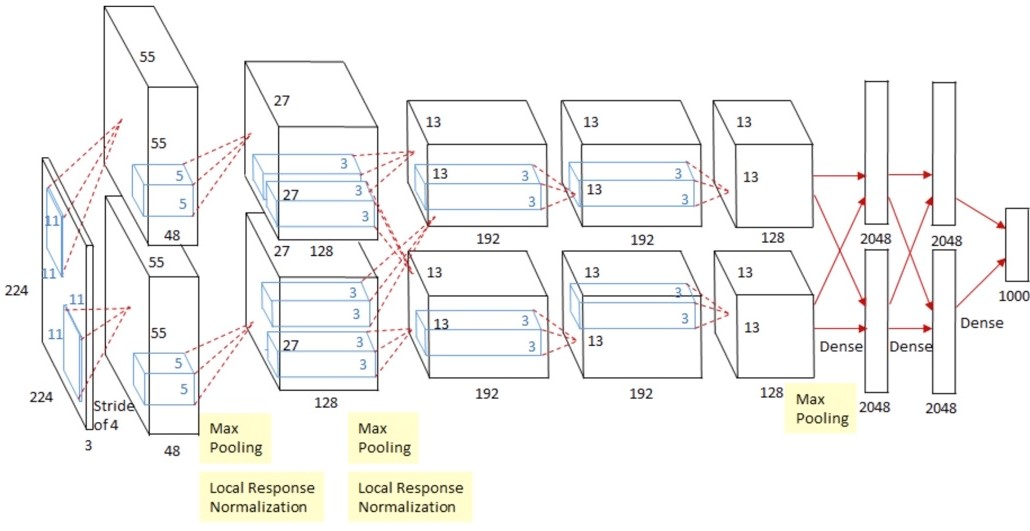
\includegraphics[width=1.0\linewidth]{AlexNet.jpeg}\
    \captionsetup{format=hang}
    \caption{Architektura sieci \emph{AlexNet} zaprezentowana w~2012 roku przez Alexa Krizhevsky'ego, Ilya Sutskevera i Geoffrey'a Hintona \cite{alexnet}}
    \label{fig:alexnet1}
\end{figure}

Sieć stworzona przez Krizhevsky'ego, Sutskevera i~Hintona  swoją architekturą bardzo przypominała sieć \emph{LeNet-5}, była jednak od niej wielokrotnie większa pod względem liczby parametrów. Składała się ona bowiem z~około 60 milionów trenowalnych parametrów podzielonych na osiem warstw (pięć warstw konwolucyjno-grupujących i~trzy warstwy gęste) o~filtrach rozmiarów 11 x 11, a~jako wejście przyjmowała obrazy RGB o~rozdzielczości 224~x~224 (patrz rysunek \ref{fig:alexnet1}). Sieć ta jest obecnie powszechnie znana pod nazwą \textbf{\emph{AlexNet}} (od imienia jej głównego autora), wygrała ona w~2012 roku prestiżowy konkurs \emph{ImageNet Large Scale Visual Recognition Challenge} pokonując drugi najlepszy model o~ponad 10~punktów procentowych (pod kątem stopy błędów top-5), zapoczątkowując tym samym swoistą rewolucję w dziedzinie głębokiego uczenia.

\paragraph*{VGGNet}

Kolejnym istotnym modelem z~perspektywy rozwoju głębokich sieci neuronowych był model \textbf{\emph{VGGNet}} zaprojektowany w~2014 roku przez Karen Simonyan i Andrew Zissermana. W~swoim artykule \emph{Very deep convolutional networks for large-scale image recognition} \cite{simonyan} zaproponowali oni konwolucyjną sieć neuronową o~niespotykanej dotąd głębokości liczącej 19 warstw i~o~filtrach wielkości 3 x 3 (patrz rysunek \ref{fig:vggnet1}). Użycie tak małych filtrów, autorzy argumentowali tym, iż zastosowanie modułu składającego się z~trzech filtrów 3 x 3, ma efektywne pole postrzegania jak jeden filtr 7 x 7, za to wymaga zdecydowanie mniejszej liczby trenowalnych parametrów i~pozwala zastosować trzykrotnie funkcję aktywacji. Pomimo tych zabiegów sieć \emph{VGGNet} posiadała bardzo duże rozmiary - składała się bowiem z~około 144 milionów trenowalnych parametrów.

\begin{figure}[!h]
    \centering 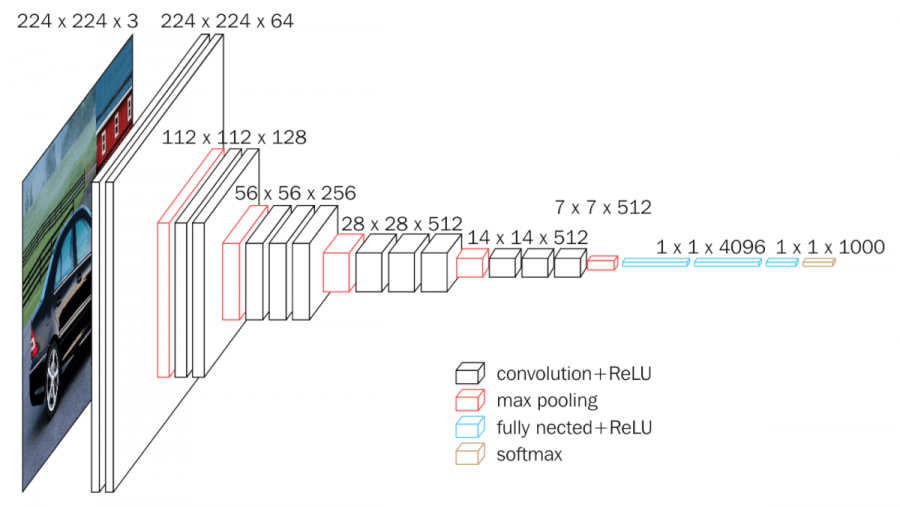
\includegraphics[width=1.0\linewidth]{VGGNet.png}
    \captionsetup{format=hang}
    \caption{Architektura sieci \emph{VGGNet} zaprezentowana w~2014 roku przez Karen Simonyan i~Andrew Zissermana \cite{simonyan}}
    \label{fig:vggnet1}
\end{figure}

\paragraph*{GoogleNet}

Sieć \emph{VGGNet} zajęła drugie miejsce w~konkursie \emph{ImageNet Large Scale Visual Recognition Challenge 2014} osiągając stopę błędów top-5 na poziomie 7,32\%. Pierwsze miejsce w~tym konkursie zajęła sieć \textbf{\emph{GoogleNet}}, osiągając wynik równy 6,67\%. Sieć ta została zaproponowana w~październiku 2014 roku przez Szegedy Ch., Liu W., Jia Y., Sermanet P., Reed S., Anguelov D., Erhan D., Vanhoucke V., Rabinovich A. w~artykule \emph{Going deeper with convolutions}. Do momentu powstania \emph{GoogleNet} większość głębokich sieci neuronowych była realizowana przy pomocy sekwencyjnego nakładania na siebie warstw splotowych i~grupujących, sieć zaprojektowana przez pracowników \emph{Google Inc.} jako pierwsza wprowadziła przetwarzanie równoległe realizowane w blokach \emph{Inception}. Bloki te były realizowane jako równolegle warstwy konwolucyjne o~filtrach różnych rozmiarów (\textit{1x1}, \textit{3x3}, \textit{5x5}), których wynik był scalany (przy pomocy operacji konkatenacji) w~jedną warstwę na wyjściu z~danego bloku (patrz rysunek\ref{fig:inception1}). Zastosowanie w~blokach \emph{Inception} filtrów o~kilku różnych rozmiarach miało umożliwić detekcję cech o~dużym zróżnicowaniu przestrzennym. Zastosowanie filtrów  \textit{3x3}~służyło redukcji złożoności sieci, dzięki czemu finalny model zawierał około pięć milionów trenowalnych parametrów, czyli mniej więcej 12~razy mniej niż dużo mniej efektywna sieć \emph{AlexNet} z~2012 roku. Cała architektura modelu \emph{GoogleNet} składała się z~22~połączonych ze sobą sekwencyjnie bloków, z~czego dziewięć stanowiły moduły \emph{Inception}, łącznie w~całej sieci można było wyróżnić około 100~różnych warstw (patrz rysunek \ref{fig:googlenet1}).

\begin{figure}[!h]
    \centering 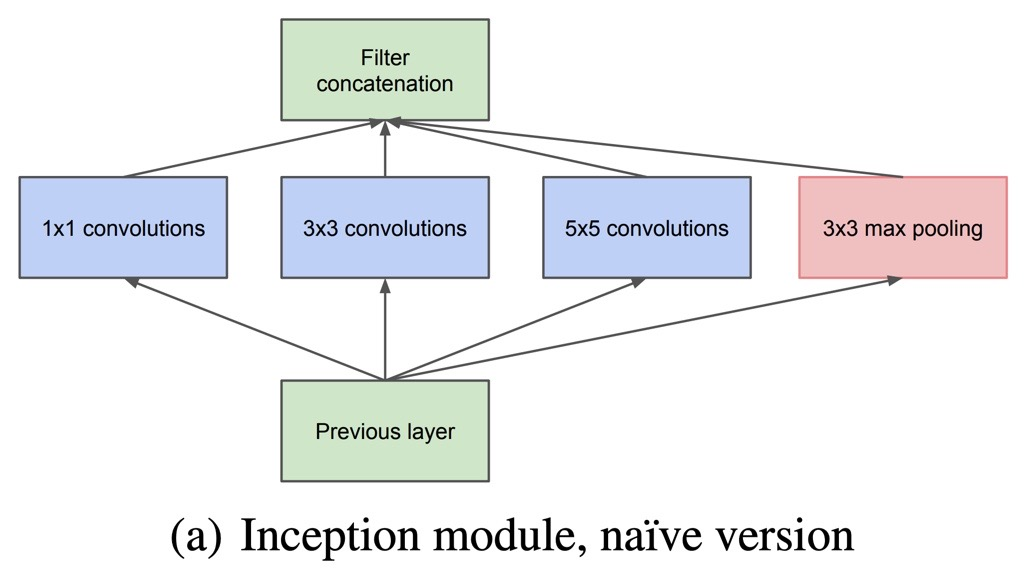
\includegraphics[width=0.8\linewidth]{Inception1.jpeg}
    \centering 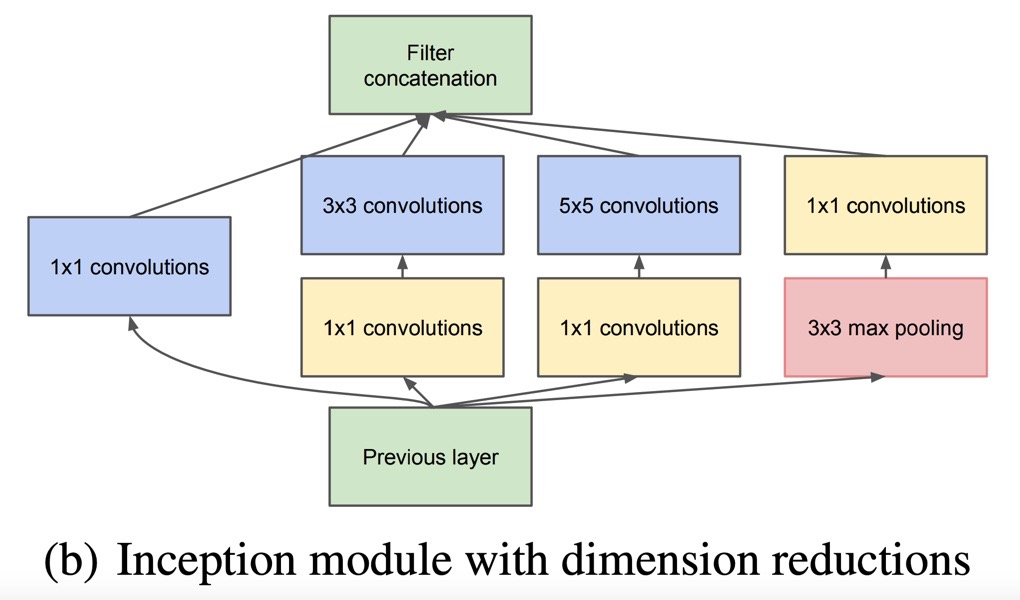
\includegraphics[width=0.8\linewidth]{Inception2.jpeg}
    \captionsetup{format=hang}
    \caption{Architektura bloku \emph{Inception} zaprezentowana w~2014 roku w~artykule \emph{Going deeper with convolutions} \cite{szegedy}}
    \label{fig:inception1}
\end{figure}

 W~kolejnych latach autorzy modelu \emph{GoogleNet} wprowadzili liczne poprawki do opisywanej przez siebie architektury, dodali m.in. operację normalizacji partiami, faktoryzację konwolucji w~celu poprawienia efektywności obliczeniowej, usprawnili architekturę bloków \emph{Inception} poprzez dodanie połączeń \emph{residual connections} oraz zastosowali konwolucje separowalne wgłębnie (ang. \emph{depthwise separable convolutions}) i~punktowo (ang/ \emph{pointwise separable convolutions}) W~ten sposób powstały kolejne, jeszcze bardziej skuteczne, architektury wyrastające wprost z~\emph{GoogleNet} (zwanej też \emph{Inception-v1}), były nimi: \emph{Inception-v2} [2015], \emph{Inception-v3} [2015], \emph{Inception-v4} [2016] oraz \emph{Xception} [2017].

\newpage
\begin{figure}[!h]
    \centering 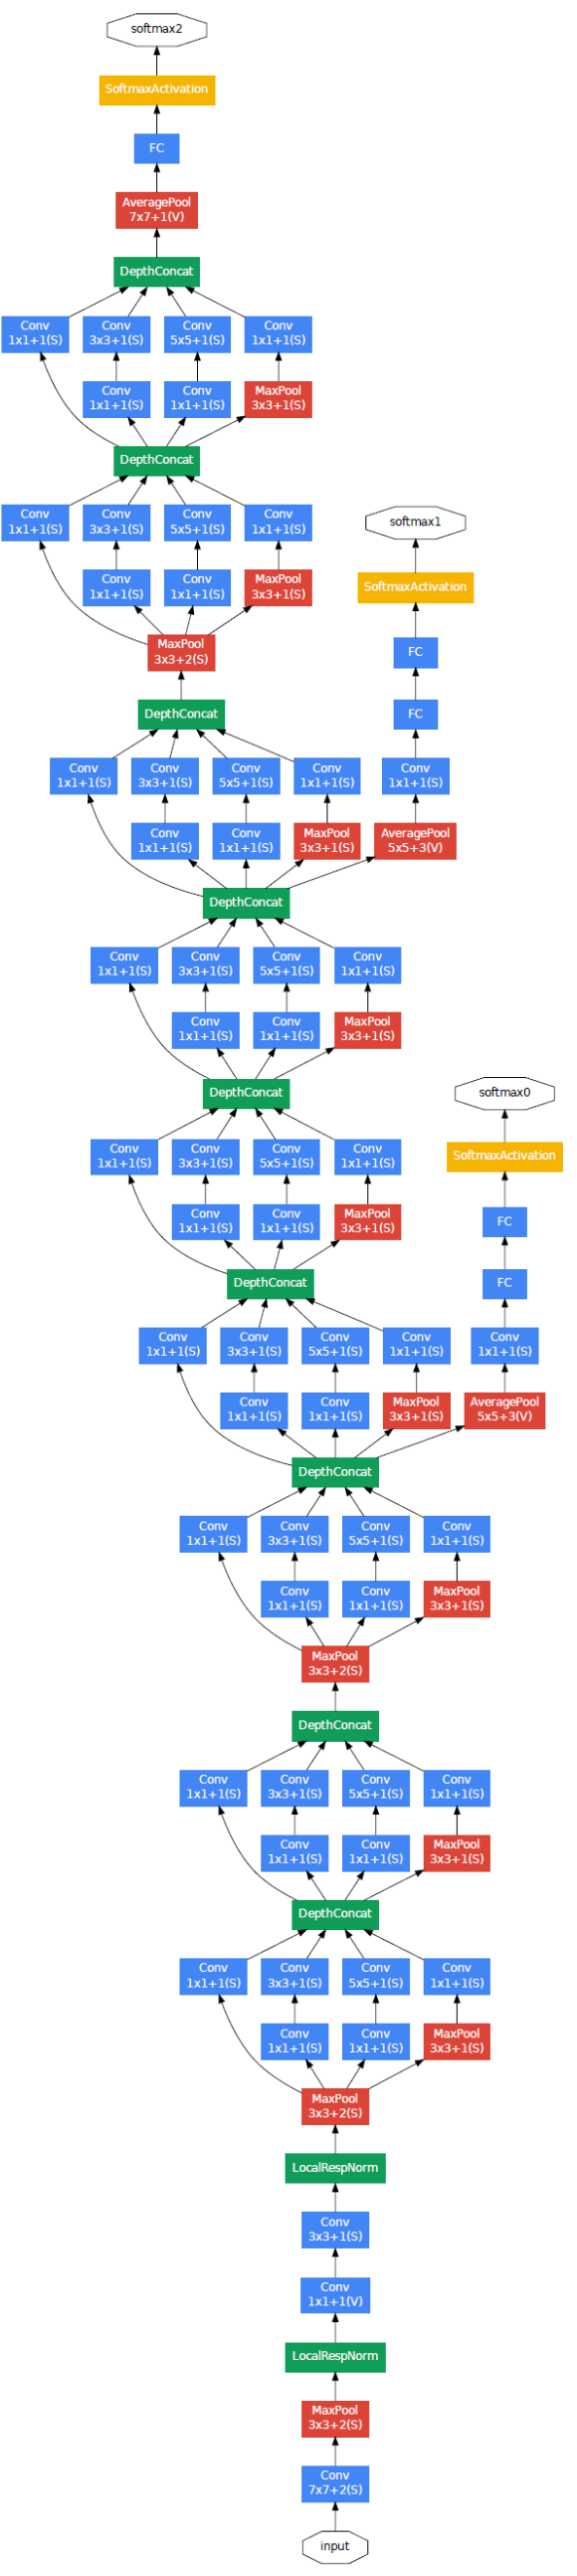
\includegraphics[width=0.32\linewidth]{GoogleNet.png}
    \captionsetup{format=hang}
    \caption{Architektura sieci \emph{GoogleNet} zaprezentowana w~2014 roku w~artykule \emph{Going deeper with convolutions} \cite{szegedy}}
    \label{fig:googlenet1}
\end{figure}
\newpage

\paragraph*{Generative Adversarial Nets (GAN)}

W~czasie gdy konwolucyjne sieci neuronowe ewoluowały w~stronę coraz większej liczby warstw i~coraz większej głębokości, naukowcy z~Uniwersytetu w~Montrealu: Goodfellow I., Pouget-Abadie J., Mirza M., Xu B., Warde-Farley D.,
Ozair S., Courville A. i~Bengio Y. w~swojej pracy z~2014~roku pod tytułem \emph{Generative Adversarial Nets} \cite{goodfellow} zaproponowali zupełnie nową architekturę głębokich sieci neuronowych określanych mianem sieci generatywnych z~adwersarzem - \textbf{\emph{GAN}}. W~ramach \emph{GAN} jednoczenie trenowane są dwa modele: 

\begin{itemize}
\item model generatywny (ang. \emph{generative model}), który stara się odwzorować dystrybucję danych w~zbiorze treningowym, tak, żeby zmaksymalizować prawdopodobieństwo, że dyskryminator popełni błąd,
\item model dyskryminacyjny (ang. \emph{discriminative model}), który szacuje prawdopodobieństwo, że próbka pochodzi z~danych uczących, a~nie z~generatora.
\end{itemize}

\begin{figure}[!h]
    \centering 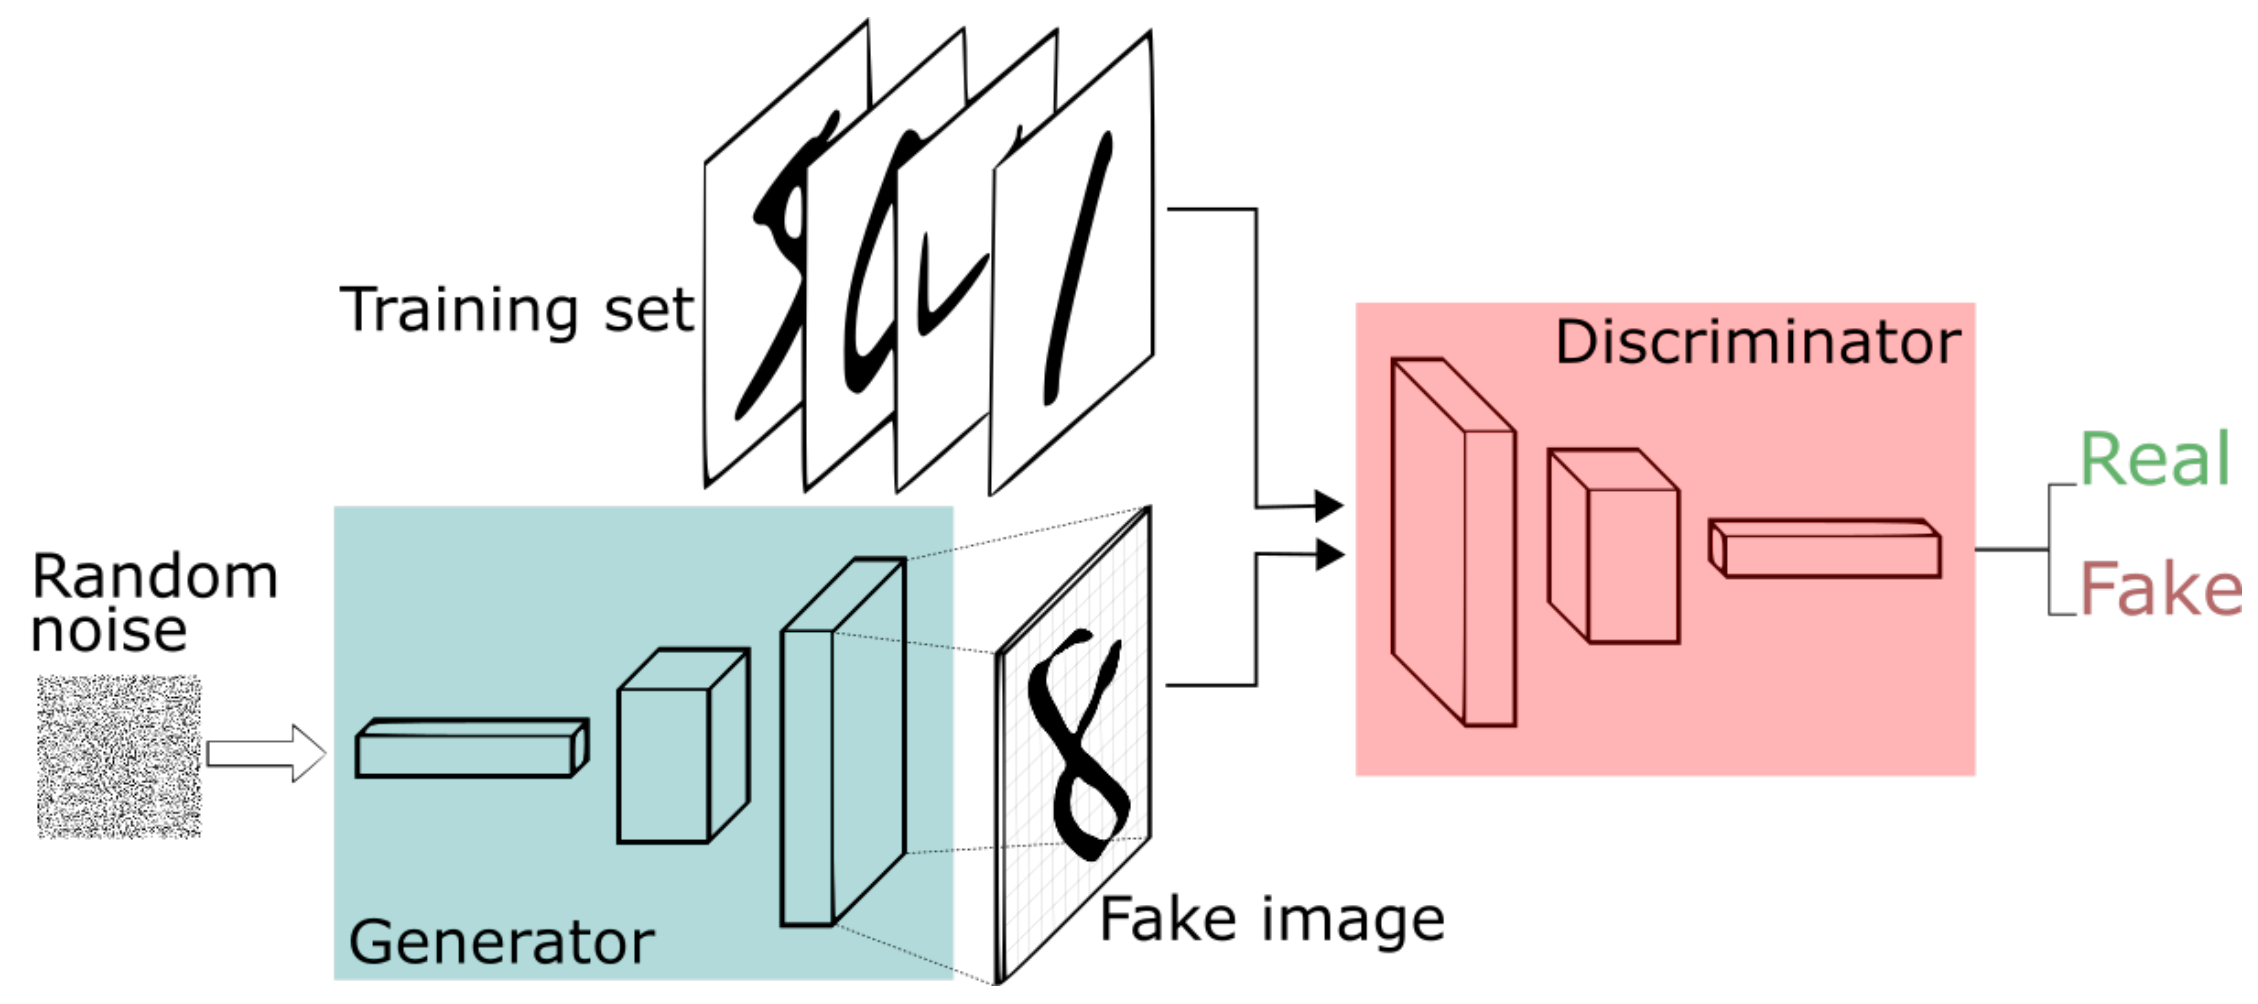
\includegraphics[width=0.7\linewidth]{GAN.png}
    \captionsetup{format=hang}
    \caption{Wizualizacja architektury modelu GAN (Źródło: \url{https://jrmerwin.github.io/deeplearning4j-docs/generative-adversarial-network.html})}
    \label{fig:gan1}
\end{figure}

W~ten sposób pomiędzy generatorem a~dyskryminatorem dochodzi do gry o~sumie zerowej, której celem jest jak najlepsze wytrenowanie generatora w~ekstrakcji i~odwzorowaniu cech ze zbioru treningowego. \emph{GAN} jest dobrym przykładem uczenia nienadzorowanego (ang. \emph{unsupervised learning}), które w~przeciwieństwie do uczenie nadzorowanego (ang. \emph{supervised learning}) nie potrzebuje posiadać w~zbiorze treningowym etykiet wskazujących jaki jest oczekiwany wynik, który ma zostać wygenerowany przez model. 

\paragraph*{Region Based Convolutional Neural Networks (R-CNN)}

Rok 2014 był bardzo istotnym rokiem w~dziejach rozwoju głębokich sieci neuronowych, gdyż w~tym właśnie roku poza tak istotnymi architekturami jak \emph{VGGNet}, \emph{GoogleNet} czy \emph{GAN}, powstała jeszcze jedna bardzo ważna architektura o nazwie \emph{Region Based Convolutional Neural Networks} (\textbf{\emph{R-CNN}}). Została ona zaproponowana przez Rossa Girshicka, Jeffa Donahue'a, Trevora Darrella i~Jitendra Malika w~artykule \emph{Rich feature hierarchies for accurate object detection and semantic segmentation} \cite{girshick}. Celem sieci \emph{R-CNN} była detekcja obiektów na zdjęciach, czyli nie tylko wskazanie, że na danym zdjęciu jest określony obiekt, ale też zaznaczanie przy pomocy ramki, gdzie dokładnie dany obiekt się znajduje (patrz rysunek \ref{fig:rcnn1})

\begin{figure}[!h]
    \centering 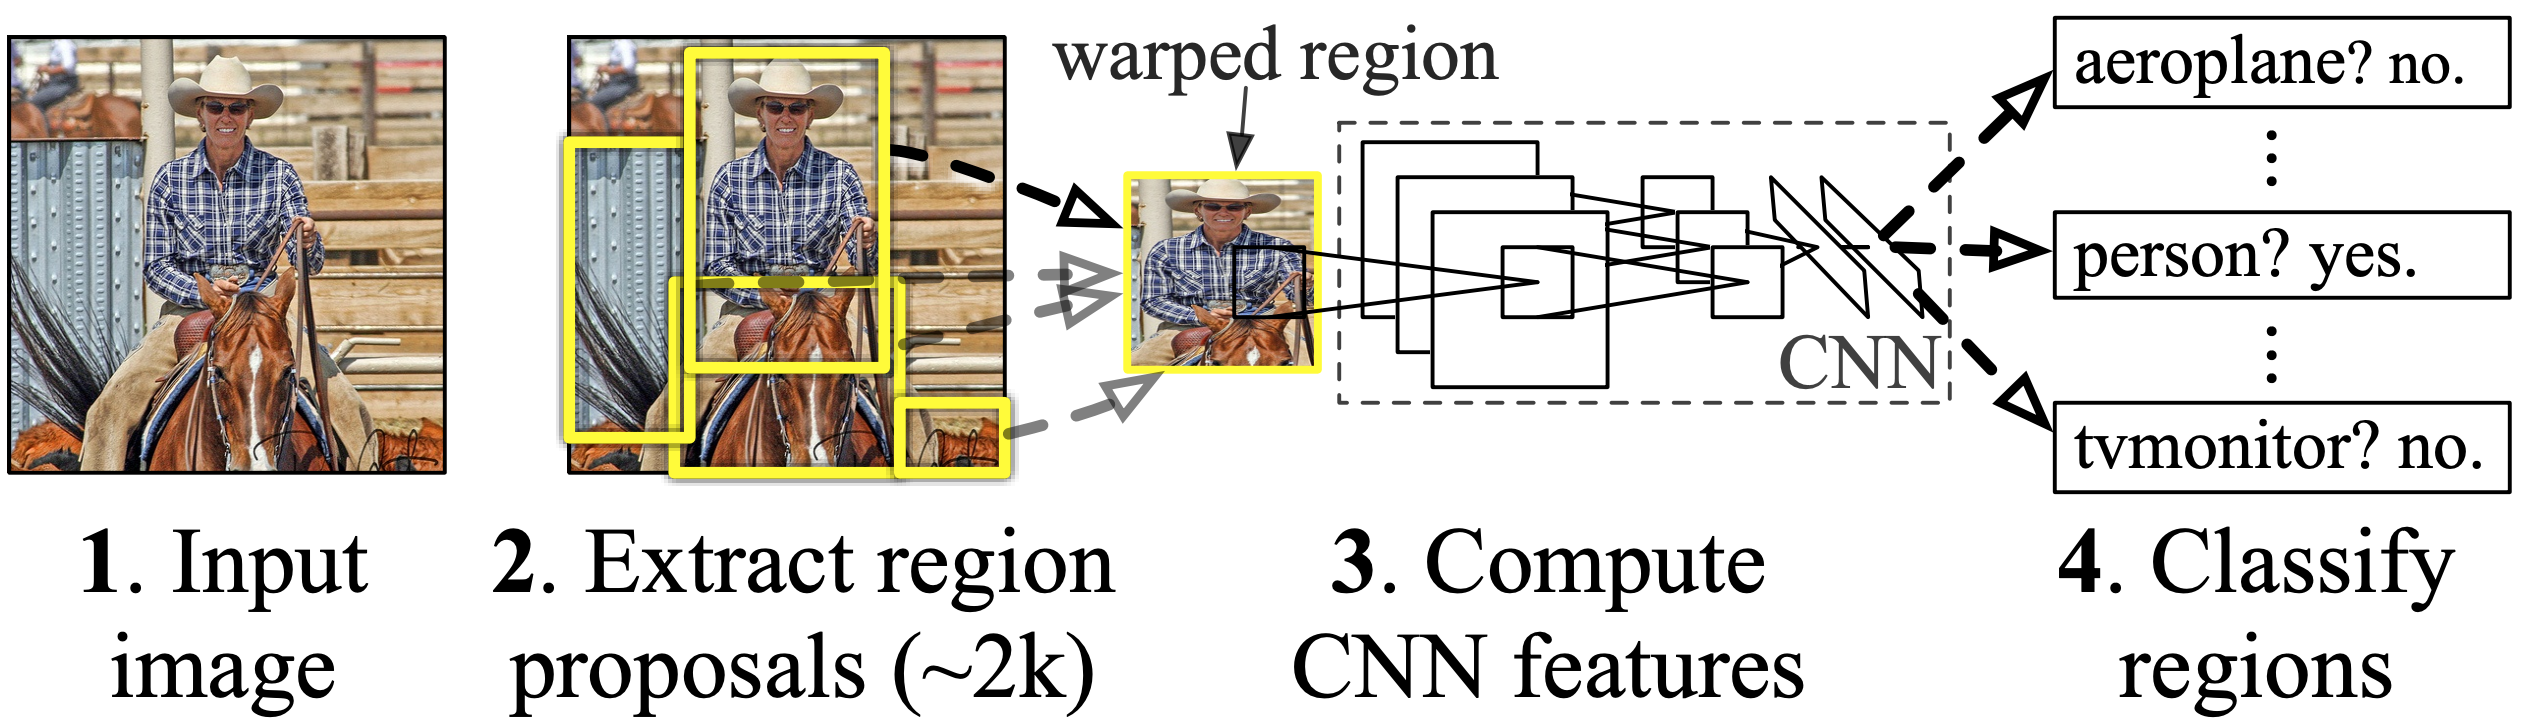
\includegraphics[width=1.0\linewidth]{R-CNN.png}
    \captionsetup{format=hang}
    \caption{Schemat działania modelu \emph{R-CNN} zaprezentowany w~2014~roku przez Rossa Girshicka, Jeffa Donahue'a, Trevora Darrella i~Jitendra Malika \cite{girshick}}
    \label{fig:rcnn1}
\end{figure}

Oryginalna sieć \emph{R-CNN} bazowała na algorytmie o nazwie \emph{Selective Search}, który dzielił obraz wejściowy na około dwa tysiące regionów zainteresowania (ang. \emph{regions of interest}), które następnie były przepuszczone przez konwolucyjną sieć neuronową, która ekstraktowała najważniejsze cechy danego \emph{ROI} i~przydzielała obiekt, który znajdował się w~danym regionie, do odpowiedniej kategorii. Taka konstrukcja sieci \emph{R-CNN} miała jednak wiele wad - wieloetapowość, nieefektywność obliczeniową czy bardzo wolne działanie (detekcja obiektów na jednym obrazie trwała około 47~sekund). Stąd też w~kolejnych latach autorzy oryginalnego artykułu zaproponowali bardziej efektywne obliczeniowo implementacje \emph{R-CNN}:

\begin{itemize}
\item sieć \emph{Fast R-CNN} [2015] - była rozwinięciem sieci \emph{R-CNN}, w~którym konwolucyjna sieć neuronowa nie ekstraktowała cech z~poszczególnych regionów zainteresowania tylko z~całego obrazu wejściowego a~algorytm \emph{Selective Search} był stosowany dopiero na wyekstraktowanych mapach cech, co znacząco przyspieszyło działanie sieci, gdyż ekstrakcja cech przy pomocy sieci \emph{CNN} miała miejsce tylko jeden raz (zamiast dwóch tysięcy razy),
\item sieć \emph{Faster R-CNN} [2016] - była rozwinięciem \emph{Fast R-CNN}, w~którym  algorytm \emph{Selective Search} został zastąpiony przez oddzielną sieć neuronową, która uczyła się przewidywania regionów zainteresowania,
\end{itemize}

Obie powyższe implementacje znacząco przyspieszyły detekcję obiektów - sieć \emph{Fast R-CNN} była ponad 20~razy, a sieć \emph{Faster R-CNN} ponad 200 razy, szybsza w~detekcji obiektów niż oryginalna sieć \emph{R-CNN}.  Uzyskanie tak dużej efektywności sieci \emph{Faster R-CNN} sprawiło, iż mogła ona być stosowana do detekcji obiektów w~czasie rzeczywistym (ang. \emph{real-time object detection}).

\paragraph*{ResNet}

W~2015 roku konkurs \emph{ILSVRC} wygrał model konwolucyjny o~niespotykanej dotąd głębokości 152~warstw - był to model zaprojektowany przez pracowników \emph{Microsoft Research Asia} o~nazwie \textbf{\emph{ResNet}}. Na zbiorze \emph{ImageNet} osiągnął on fenomenalną stopę błędów top-5 równą 3,57\%, uzyskując tym samym nadludzką skuteczność (dla przeciętnego człowieka stopa błędów na tym zbiorze wynosi około 5\%). Autorami tego sukcesu byli He K., Zhang X., Ren S. i~Sun J., którzy w~swoim artykule \emph{Deep Residual Learning for Image Recognition} z~2015 roku \cite{he} zaprezentowali efektywną metodę radzenia sobie z~problemem zanikającego gradientu w~bardzo głębokich sieciach neuronowych. Rozwiązaniem zaproponowanym przez pracowników \emph{Microsoft Research Asia} był blok rezydualny (ang. \emph{residual block}), który był realizowany przy pomocy połączeń rezydualnych (ang. \emph{residual (skip) connections}) zakończonych operacją sumowania. Połączenia te, pomijając niektóre warstwy konwolucyjno-aktywacyjne, przekazywały gradient błędu bezpośrednio do wyższych warstw sieci w~ten sposób zachowując istotny wpływ na zmienność ich wag (patrz rysunek \ref{fig:residual1}). Zwycięska sieć \emph{ResNet-152}\footnote{Liczba przy nazwie sieci \emph{ResNet} wskazuje z~ilu warstw dana sieć rezydualna się składa.} miała około 60~milionów trenowalnych parametrów, czyli o ponad połowę mniej niż sieć \emph{VGGNet}, ale za to kilkakrotnie razy więcej niż sieć \emph{GoogleNet}.

\begin{figure}[!h]
    \centering 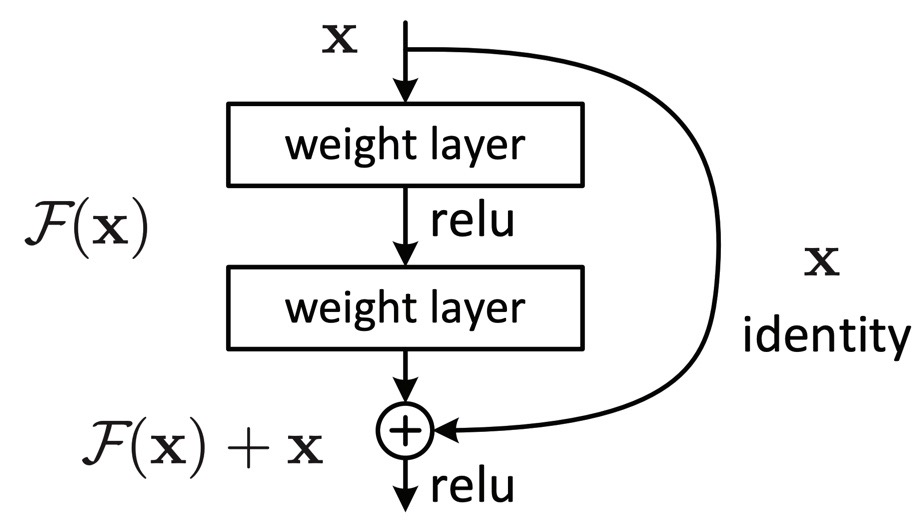
\includegraphics[width=0.8\linewidth]{Residual.jpeg}
    \captionsetup{format=hang}
    \caption{Blok rezydualny zaprezentowany w~2015 roku przez He K., Zhang X., Ren S. i~Sun J. \cite{he}}
    \label{fig:residual1}
\end{figure}

Sieć \emph{ResNet-152} doczekała się licznych modyfikacji w~kolejnych latach, w~których to była ona uzupełniana między innymi o:~bloki wzorowane na blokach \emph{Inception} sieci \emph{GoogleNet} (\emph{Inception-v4} [2016], \emph{ResNext} [2017], \emph{Wide ResNet} [2017]), większą liczbę połączeń rezydualnych (\emph{DenseNet} [2016]) czy po prosu większą liczbę warstw (\emph{ResNet-1202} [2015], \emph{ResNet-164} [2016]).

\newpage
\begin{figure}[!h]
    \centering 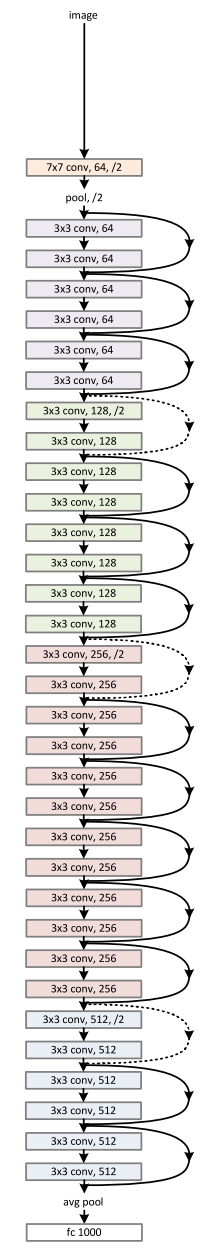
\includegraphics[width=0.23\linewidth]{ResNet.png}
    \captionsetup{format=hang}
    \caption{Przykładowa architektura sieci \emph{ResNet-34} zaprezentowana w~2015~roku przez He K., Zhang X., Ren S. i~Sun J. \cite{he}}
    \label{fig:resnet1}
\end{figure}
\newpage

\paragraph*{U-Net}

W~tym samym roku co sieć \emph{ResNet} zaprezentowana została inna konwolucyjna sieć neuronowa o~bezprecedensowej dotąd architekturze - w~kształcie litery „U”. Sieć ta zyskała nazwę \textbf{\emph{U-Net}} i~została szczegółowo opisana przez Olafa Ronnebergera, Philippa Fischera i~Thomasa Broxa w~artykule \emph{U-Net: Convolutional Networks for Biomedical Image Segmentation} \cite{ronneberger}. Sieć \emph{U-Net} składa się z~dwóch części:
\begin{itemize}
\item enkodera, w~ramach którego przy pomocy warstw splotowo-grupujących następuje ekstrakcja cech wejściowego obrazu na różnych poziomach rozdzielczości przestrzennej (ścieżka analizy),
\item dekodera, w~ramach którego przy pomocy nadpróbkowania (ang. \emph{upsamoling}) następuje propagacja informacji kontekstowej do warstw o~wyższej rozdzielczości przestrzennej (ścieżka syntezy),
\end{itemize}

\begin{figure}[!h]
    \centering 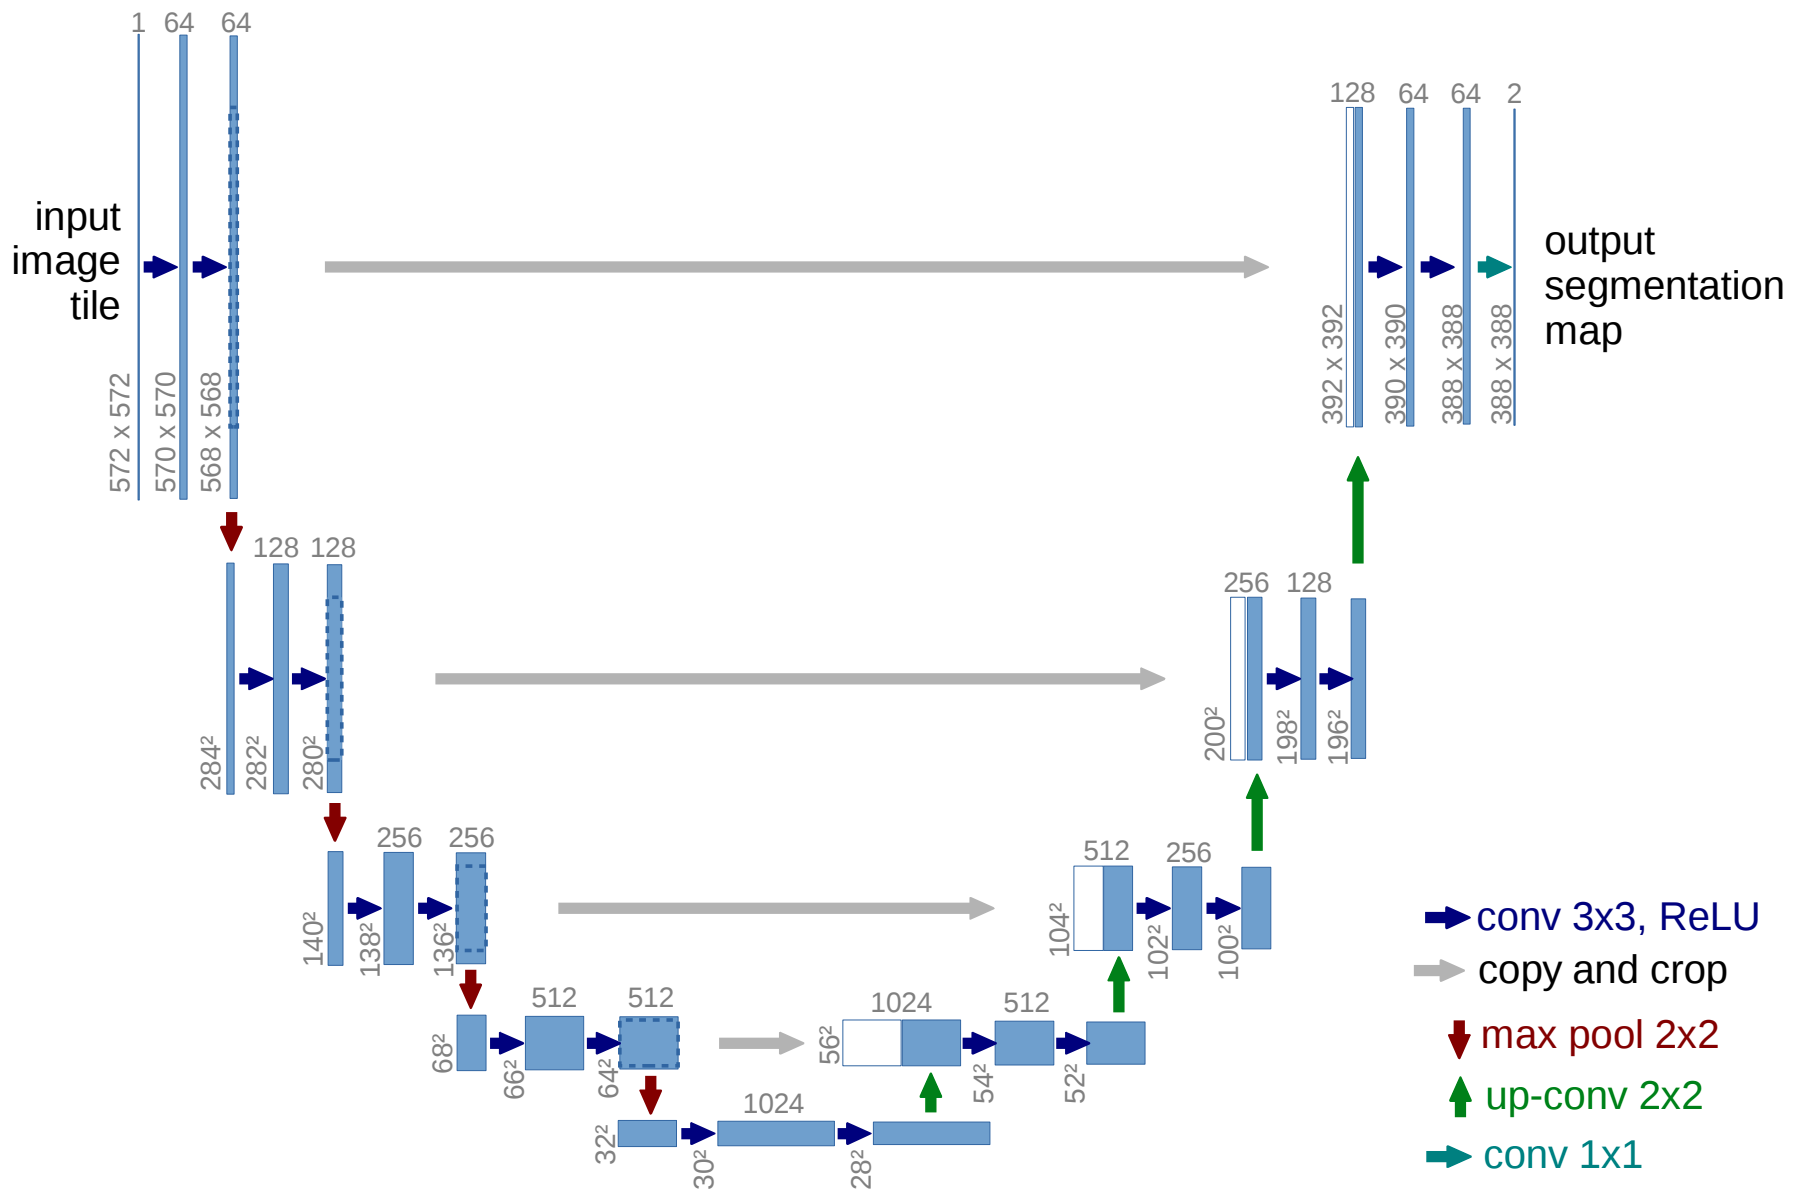
\includegraphics[width=0.8\linewidth]{U-Net.png}
    \captionsetup{format=hang}
    \caption{Architektura sieci \emph{U-Net} zaprezentowana w~2015 roku przez Olafa Ronnebergera, Philippa Fischera i~Thomasa Broxa \cite{ronneberger}}
    \label{fig:unet1}
\end{figure}

Pomiędzy każdą z~warstw enkodera i~dekodera, w architekturze \emph{U-Net} występują bezpośrednie połączenia rezydualne\footnote{W~odróżnieniu od sieci \emph{ResNet}, połączenia rezydualne w~sieci \emph{U-Net} były finalizowane przy pomocy operacji konkatenacji z~warstwami dekodera (jak w~blokach \emph{Inception}), a~nie operacji sumowania (jak w~blokach rezydualnych)}, które transferują informacje z~niskich warstw enkodera do wysokich warstw dekodera, dzięki którym możliwa jest szczegółowa rekonstrukcja obrazu na kolejnych poziomach rozdzielczości przestrzennej. Sieć \emph{U-Net} można więc zdefiniować jako transformację w~pełni konwolucyjnej sieci neuronowej (ang. \emph{Fully Convolutional Network}), czyli konwolucyjnej sieci neuronowej niezawierającej warstw gęstych, uzupełnioną o~bezpośrednie połączenie pomiędzy ścieżką analizy a~syntezy. Sieć \emph{U-Net} była początkowo wykorzystywana przede wszystkim do semantycznej segmentacji (ang. \emph{semantic segmentation}) pikseli na zdjęciach biomedycznych, co oznacza iż jej zadaniem było przypisanie każdemu pikselowi ze zdjęcia wejściowego odpowiedniej klasy, tak aby uzyskać zdjęcie podzielone na spójne regiony odpowiadające poszczególnym klasom. Sieć ta była szczególnie efektywna w~takich zastosowaniach, gdyż nie wymagała dużej liczby danych treningowych, brakujące dane treningowe można było z~powodzeniem zastąpić augmentacją już dostępnych zdjęć. 

\paragraph*{DeepLab}

Kolejną istotną siecią neuronową szeroko stosowaną do semantycznej segmentacji obrazów, która również została zaprezentowana w~2015 roku, była sieć \textbf{\emph{DeepLab}} (znana obecnie pod nazwą \emph{DeepLabv1}). Została ona po raz pierwszy opisana w~artykule \emph{Semantic image segmentation with deep convolutional nets and fully connected CRFs} \cite{chen}, którego autorami byli Chen L., Papandreou G., Kokkinos I., Murphy K. oraz Yuille A. L. Sieć \emph{DeepLabv1} była zwykłą konwolucyjną siecią neuronową, podobnie jak \emph{U-Net} składającą się z~enkodera i~dekodera, jednak jej wyróżnikiem było zastosowanie rozszerzonych konwolucji (ang. \emph{dilated convolution} / \emph{atrous convolution})\footnote{Rozszerzone konwolucje to operacje splotowe, w~których filtr nie jest nakładany na sąsiadujące ze sobą piksele tylko na piksele oddalone od siebie o~pewną stałą odległość.}. Umożliwiają one łatwiejszą kontrolę rozdzielczości map cech oraz zapewniają większy obszar „widzenia” filtrów, co pozwala uchwycić większy zakres informacji kontekstowej. Dzięki zastosowaniu rozszerzonych konwolucji, sieć \emph{DeepLabv1} posiadała mniej trenowalnych parametrów niż inne sieci służące do semantycznej segmentacji takie jak \emph{U-Net} czy \emph{FCN} osiągając przy tym często lepsze wyniki.

\begin{figure}[!h]
    \centering 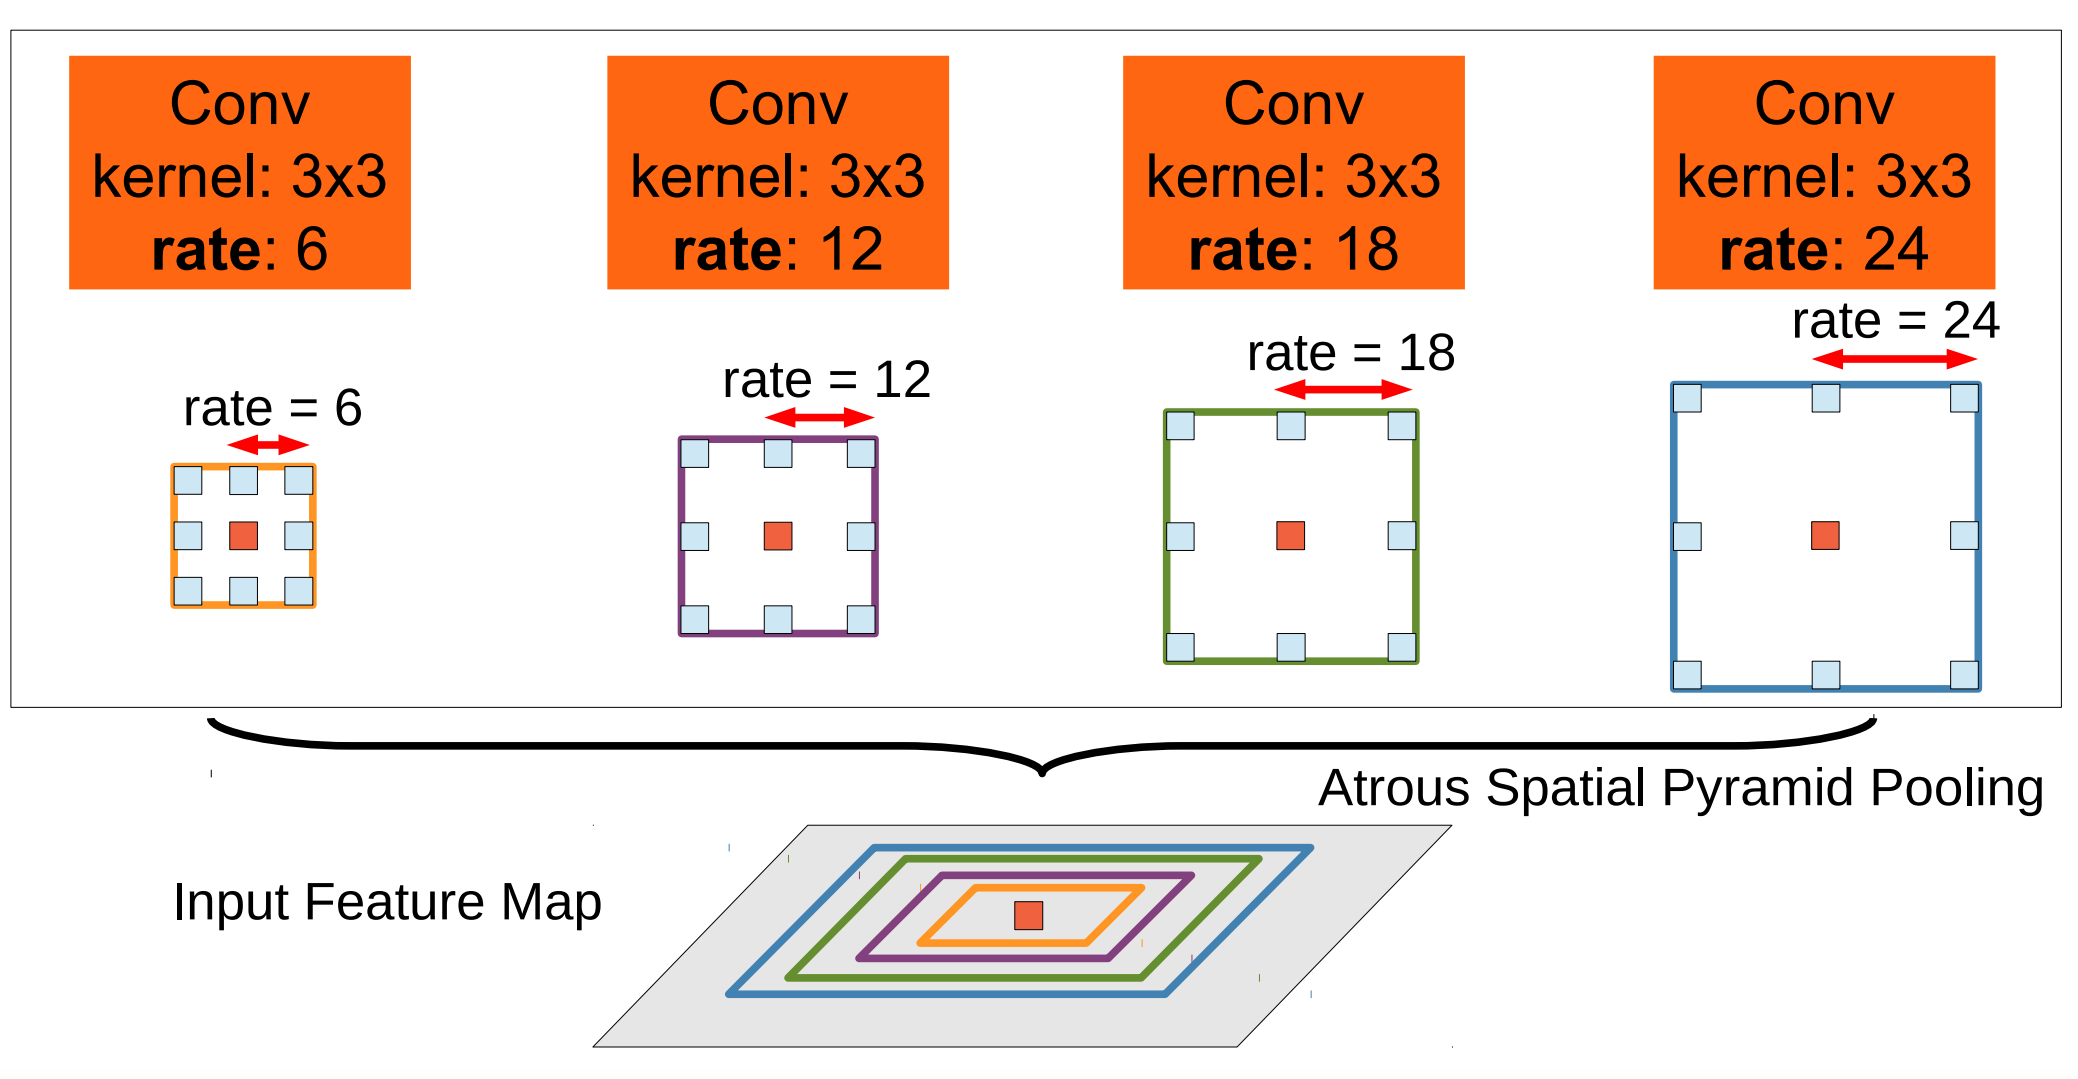
\includegraphics[width=0.9\linewidth]{ASSP.png}
    \captionsetup{format=hang}
    \caption{Architektura bloku \emph{ASSP} zaprezentowana w~2017 roku przez Chen L., Papandreou G., Kokkinos I., Murphy K. oraz Yuille A. L. \cite{chen2}}
    \label{fig:assp1}
\end{figure}

W~2017~roku autorzy sieci \emph{DeepLabv1} zaproponowali duże ulepszenie tej sieci, w~swoim artykule \emph{DeepLab: Semantic Image Segmentation with Deep Convolutional Nets, Atrous Convolution, and Fully Connected CRFs} \cite{chen2} opisali sieć \emph{DeepLabv2} wykorzystującą blok o~nazwie \emph{ASPP} (Atrous Spatial Pyramid Pooling), który zapewniał efektywną segmentację obiektów o~różnych skalach, poprzez zastosowanie rozszerzonych konwolucji z~filtrami o~różnych częstotliwościach próbkowania i~różnych efektywnych polach widzenia. Kolejne ulepszenia sieci \emph{DeepLab}, o nazwach \emph{DeepLabv3} [2017] i~\emph{DeepLabv3+} [2018], nie niosły ze sobą przełomowych rozwiązań, wprowadzały na przykład zmianę enkodera z~sieci \emph{ResNet-50}, na sieć \emph{ResNet-101}, czy dodawały konwolucje separowalne wgłębnie.

\paragraph*{You Only Look Once (YOLO)}

W~2016 roku zaprezentowany został przełomowy model w~dziedzinie rozpoznawania obiektów w~czasie rzeczywistym - \textbf{\emph{YOLO}}. Model ten przewyższał wszystkie wcześniejsze modele nie tylko pod kątem precyzji, ale także szybkości przeliczeń. Jego autorami byli Joseph Redmon, Santosh Divvals, Ross Girshick i Ali Farhadi, którzy w~swoim artykule \emph{You Only Look Once: Unified, Real-Time Object Detection} \cite{redmon} zaprezentowali konwolucyjną sieć neuronową, która jednocześnie prognozowała lokalizację obiektu (w~postaci ramki (ang. \emph{bounding box})) oraz prawdopodobieństwo klas do jakich dany obiekt według modelu należy. Model \emph{YOLO}, był w~stanie w~ciągu jednej sekundy rozpoznać obiekty na 45~zdjęciach (45~klatkach filmu), osiągając średnią precyzję (ang. \emph{mean average precision}) na poziomie 63\%.

\begin{figure}[!h]
    \centering 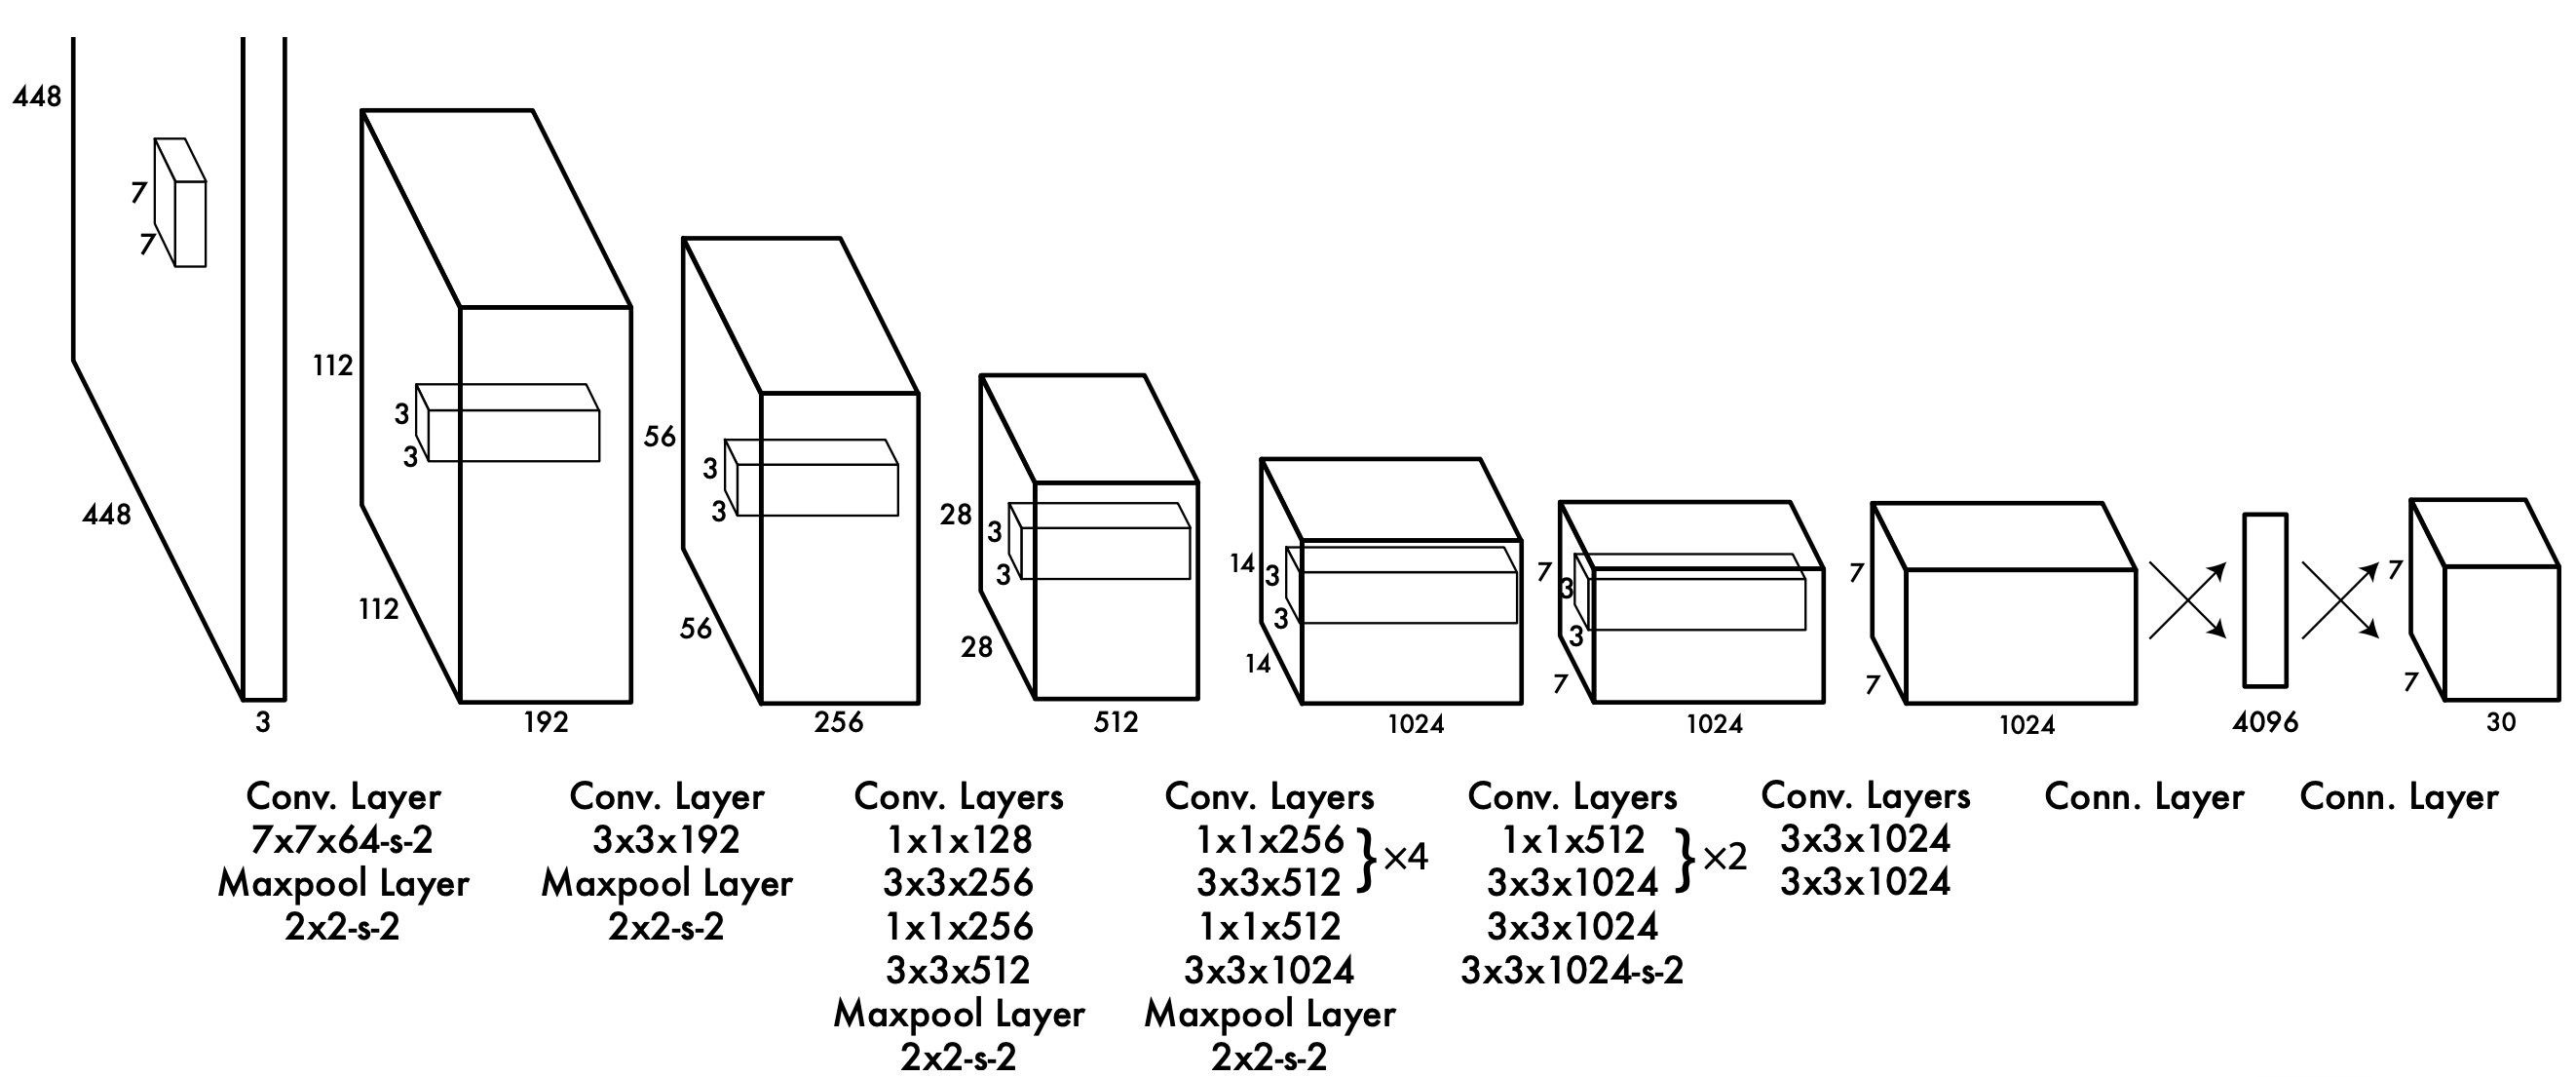
\includegraphics[width=1.0\linewidth, height=0.3\textheight]{YOLO.png}
    \captionsetup{format=hang}
    \caption{Architektura sieci \emph{YOLO} zaprezentowana w~2016 roku przez Josepha Redmona, Santosha Divvalsa, Rossa Girshicka i~Aliego Farhadiego \cite{redmon}}
    \label{fig:yolo1}
\end{figure}

Sieć stworzona przez Redmona, Divvalsa, Girshicka i~Farhadiego składała się z~24~warstw konwolucyjnych zakończonych dwoma warstwami gęstymi (patrz rysunek \ref{fig:yolo1}). Tworząc ją autorzy zainspirowali się siecią \emph{GoogleNet}, przy czym bloki \emph{inception} zostały zastąpione przez nich redukcyjnymi warstwami konwolucyjnymi  o~rozmiarze filtra 1~x~1, po których następowały warstwy z filtrami 3~x~3. Sieć \emph{YOLO} miała jednak kilka wad: nie była w~stanie efektywnie rozpoznawać bardzo małych obiektów, nie umiała efektywnie generalizować obiektów ze względu na rozmiar (jej skuteczność zależała od rozmiarów obiektów w~zbiorze treningowym) oraz miała trudności z~poprawną detekcją obiektów, które znajdowały się bardzo blisko siebie. Wszystkie te problemy zostały rozwiązane w~kolejnych wersjach modelu: \emph{YOLO v2} [2016], \emph{YOLO v3} [2018] oraz \emph{YOLO v4} [2020]. Implementacje te nie tylko rozwiązały większość problemów oryginalnej architektury, ale także poprawiły statystki pod kątem precyzji i~szybkości detekcji.

\paragraph*{Squeeze-and-Excitation Network}

W~2017~roku konkurs \emph{ImageNet Large Scale Visual Recognition Challenge} wygrała sieć \emph{Squeeze-and-Excitation Network} (\textbf{\emph{SENet}}) uzyskując stopę błędów top-5 na poziomie 2,251\% (co było o 25\% lepszym wynikiem niż najlepszy wynik z~roku 2016\footnote{Zwycięski model z 2016~roku o~nazwie \emph{Trimps-Soushen} nie został opisany w~bieżący podrozdziale, gdyż jego autorzy nie opublikowali żadnego artykułu czy raportu technicznego przedstawiającego jego architekturę.}). Autorami zwycięskiej sieci byli Hu J., Shen L., Sun G., którzy opisali ją w~swoim artykule pod tytułem \emph{Squeeze-and-Excitation Networks} \cite{hu}. Ich celem było stworzenie sieci, która położy większy nacisk na wychwycenie relacji pomiędzy kanałami obrazu wejściowego, w~miejsce relacji przestrzennych, na których skupiała się większość tworzonych w tamtym czasie modeli. Blok \emph{Squeeze-and-Excitation} zastosowany w~sieci \emph{SENet} kładzie nacisk na adaptacyjne dostosowanie wag poszczególnych kanałów, żeby odzwierciedlić istotność każdego z~nich. Jest to osiągane w~następującym procesie: warstwa grupująca do średniej (ang. \emph{average pooling}) kompresuje wszystkie kanały przestrzenne do pojedynczych wartości. Wartości te następnie uzyskują nieliniowość przez zastosowanie warstwy gęstej i~funkcji aktywacji \emph{ReLU} oraz są wygładzane przy pomocy drugiej warstwy gęstej i~funkcji aktywacji \emph{Sigmoid}. Tak przetworzone przez blok \emph{SE} wartości służą jako finalne wagi dostosowujące istotność poszczególnych kanałów przestrzennych.

\begin{figure}[!h]
    \centering 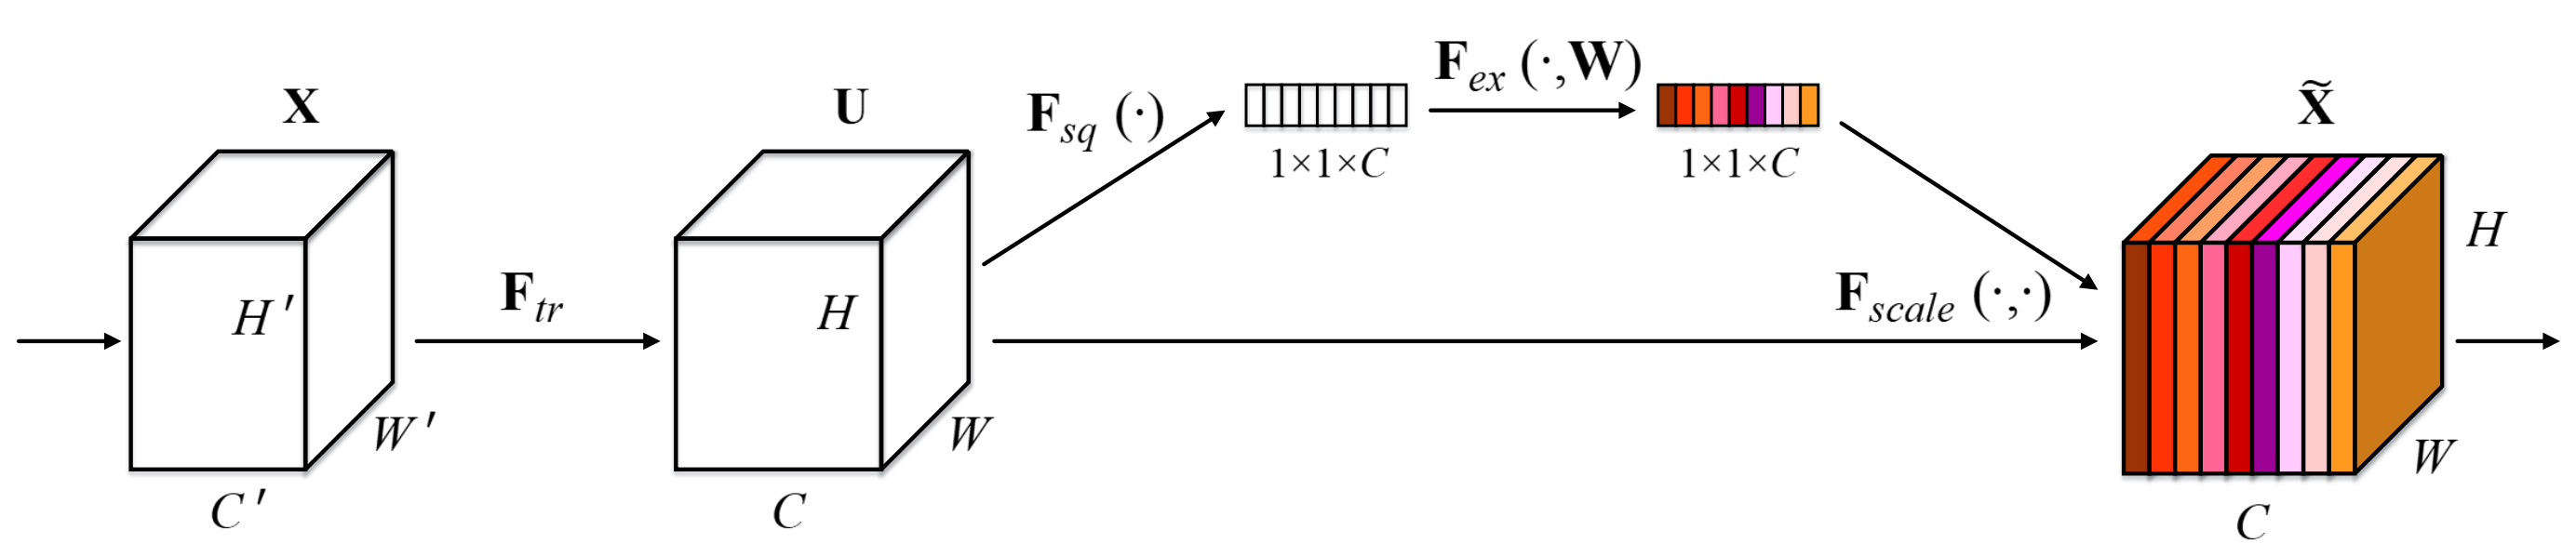
\includegraphics[width=1.0\linewidth, height=0.15\textheight]{SE.png}
    \captionsetup{format=hang}
    \caption{Architektura bloku \emph{Squeeze-and-Excitation} zaprezentowana w~2017~roku przez Hu J., Shen L. i~Sun G.\cite{hu}}
    \label{fig:se1}
\end{figure}

Prostota bloków \emph{SE} sprawia, iż mogą one być z~łatwością implementowane w~innych wiodących sieciach neuronowych. Jako przykład takiej implementacji autorzy sieci \emph{SENet} wskazywali sieć \emph{ResNet-50}, która uzupełniona o~bloki \emph{Squeeze-and-Excitation}, uzyskuje skuteczność zbliżoną do skuteczności sieci \emph{ResNet-101}, nie zwiększając istotnie liczby trenowalnych parametrów oraz kosztów obliczeniowych. Rok 2017~był ostatnim rokiem organizacji konkursu \emph{ILSVRC}  - został on zakończony, gdyż rezultaty osiągane na zbiorze testowym przez większość zgłaszanych do konkursu modeli zaczęły istotnie przekraczać wyniki przeciętnego człowieka.

\paragraph*{Capsule Neural Network (CapsNet)}

Kolejną istotną architekturą głębokich sieci neuronowych, która zostanie zaprezentowana w~bieżącym podrozdziale, jest kapsułowa sieć neuronowa (ang. \emph{capsule neural network}), która oznaczana jest skrótem \textbf{\emph{CapsNet}}. Została ona zaprezentowana w~2017 roku przez Geoffrey'a Hintona, Sarę Sabour i~Nicholasa Frossta w~artykule \emph{Dynamic Routing Between Capsules} \cite{hinton2}.

\begin{figure}[!h]
    \centering 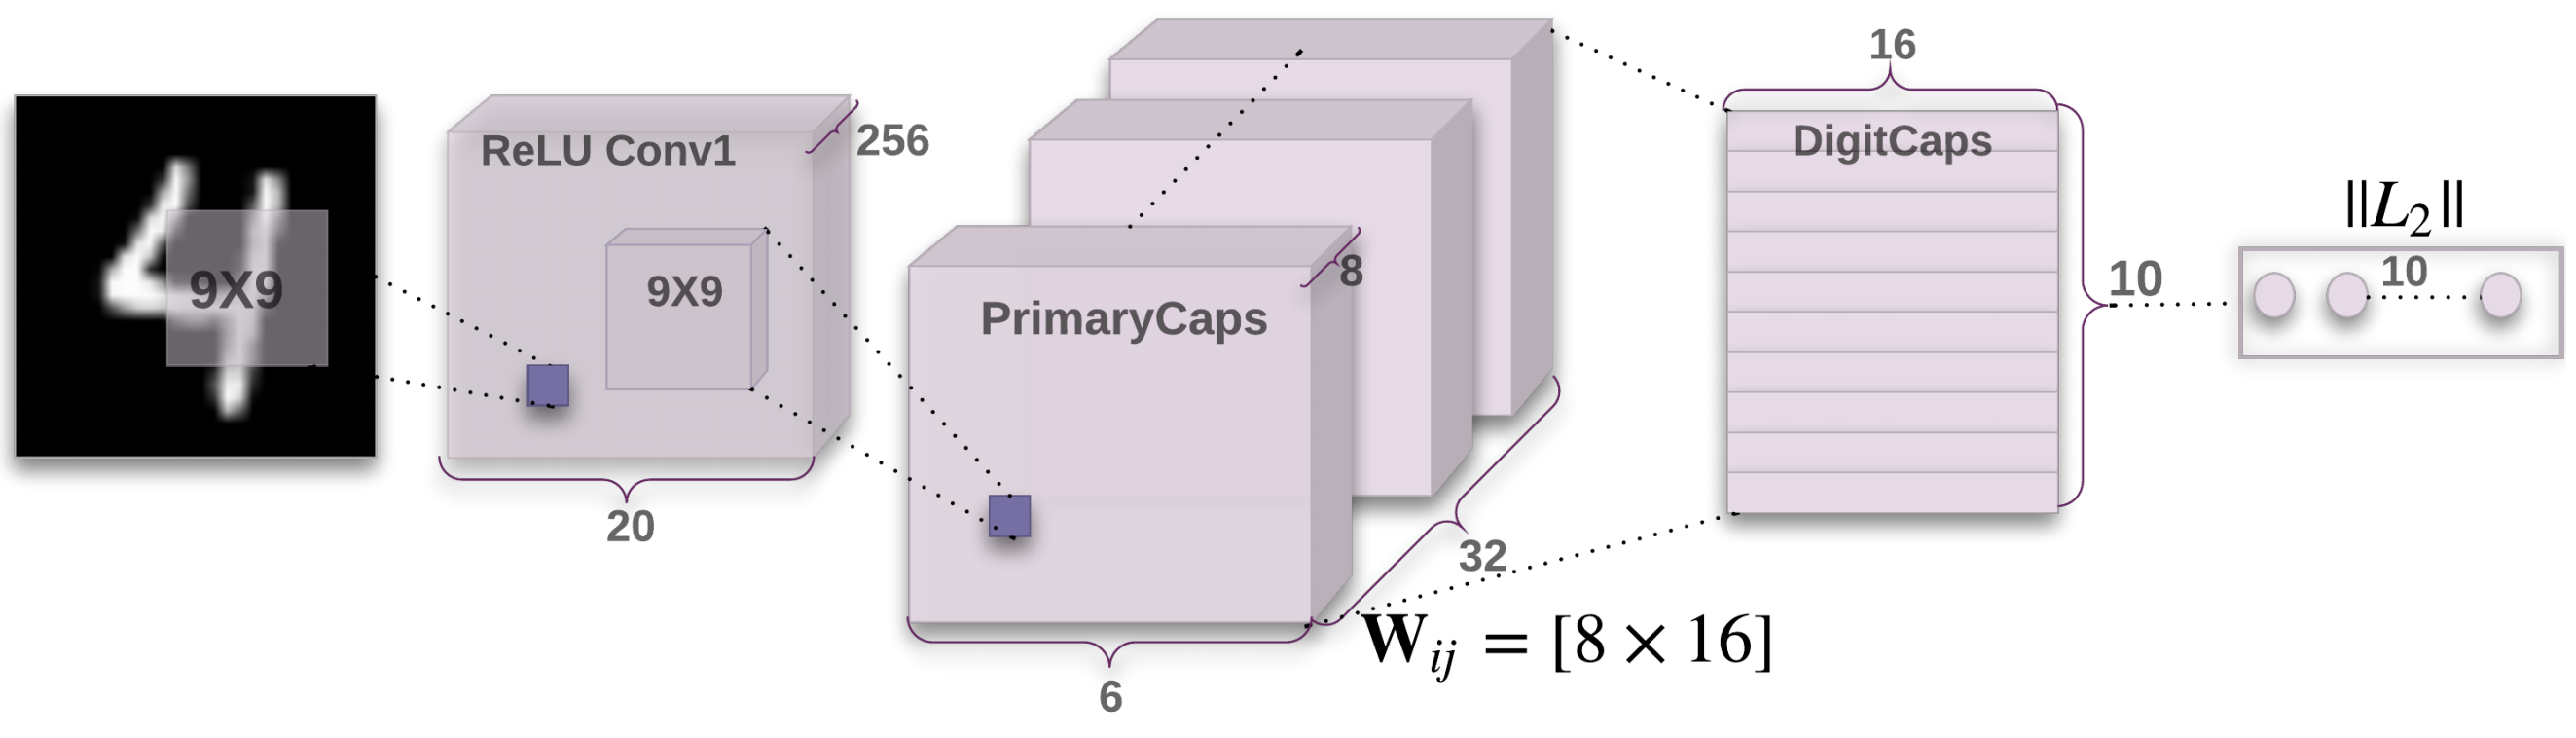
\includegraphics[width=1.0\linewidth]{capsnet.png}
    \captionsetup{format=hang}
    \caption{Architektura sieci \emph{CapsNet} zaprezentowana w~2017 roku przez Geoffrey'a Hintona, Sarę Sabour i~Nicholasa Frossta \cite{hinton2}}
    \label{fig:capsnet1}
\end{figure}

Autorzy omawianego artykułu zaproponowali dodanie do tradycyjny konwolucyjnych sieci neuronowych bloków, które nazwali kapsułami, po to by te ekstraktowały z~obrazów informacje przestrzenne (informacje dotyczące pozy) oraz prawdopodobieństwo występowania określonych obiektów na tych obrazach. Kapsuły te następnie przekazują te informacje do odpowiednich kapsuł umieszczonych powyżej nich, w~ramach procesu dynamicznego trasowania (ang. \emph{dynamic routing}), a~następnie dochodzi do zwiększenia współczynnika sprzężenia (ang. \emph{coupling coefficient}) dla kapsuł, których wyniki najsilniej rezonują z~wynikami kapsuł z~poziomu niżej oraz osłabienia tego współczynnika dla pozostałych kapsuł. W~ten sposób sieć \emph{CapsNet} adresuje problem obrazów, które składają się z~odpowiednich części, ale części te nie zachowują odpowiednich relacji przestrzennych pomiędzy sobą oraz jest w~stanie lepiej rozpoznawać obiekty, na zdjęciach robionych z~bardzo różnych kątów widzenia.


\paragraph*{Omni-Scale Network}

W~2019 roku naukowcy związani z~\emph{Samsung AI Center}, w~swojej pracy \emph{Omni-Scale Feature Learning for Person Re-Identification} \cite{zhou}, zaproponowali nowy rodzaj bloku  rezydualnego, wykorzystywanego w~ramach sieci \emph{Omni-Scale Network} (\textbf{\emph{OSNet}}), o~nazwie \emph{Bottleneck}. Blok ten był złożony z~kilku niezależnych ścieżek konwolucji, z których każda wychwytywała cechy o~innej skali. Ścieżki te były łączone przy pomocy nowatorskich bramek agregacji, które dynamicznie scalały cechy o~różnych skalach z~wagami zależnymi od kanałów wejścia (patrz rysunek \ref{fig:osblock1})

\begin{figure}[!h]
    \centering 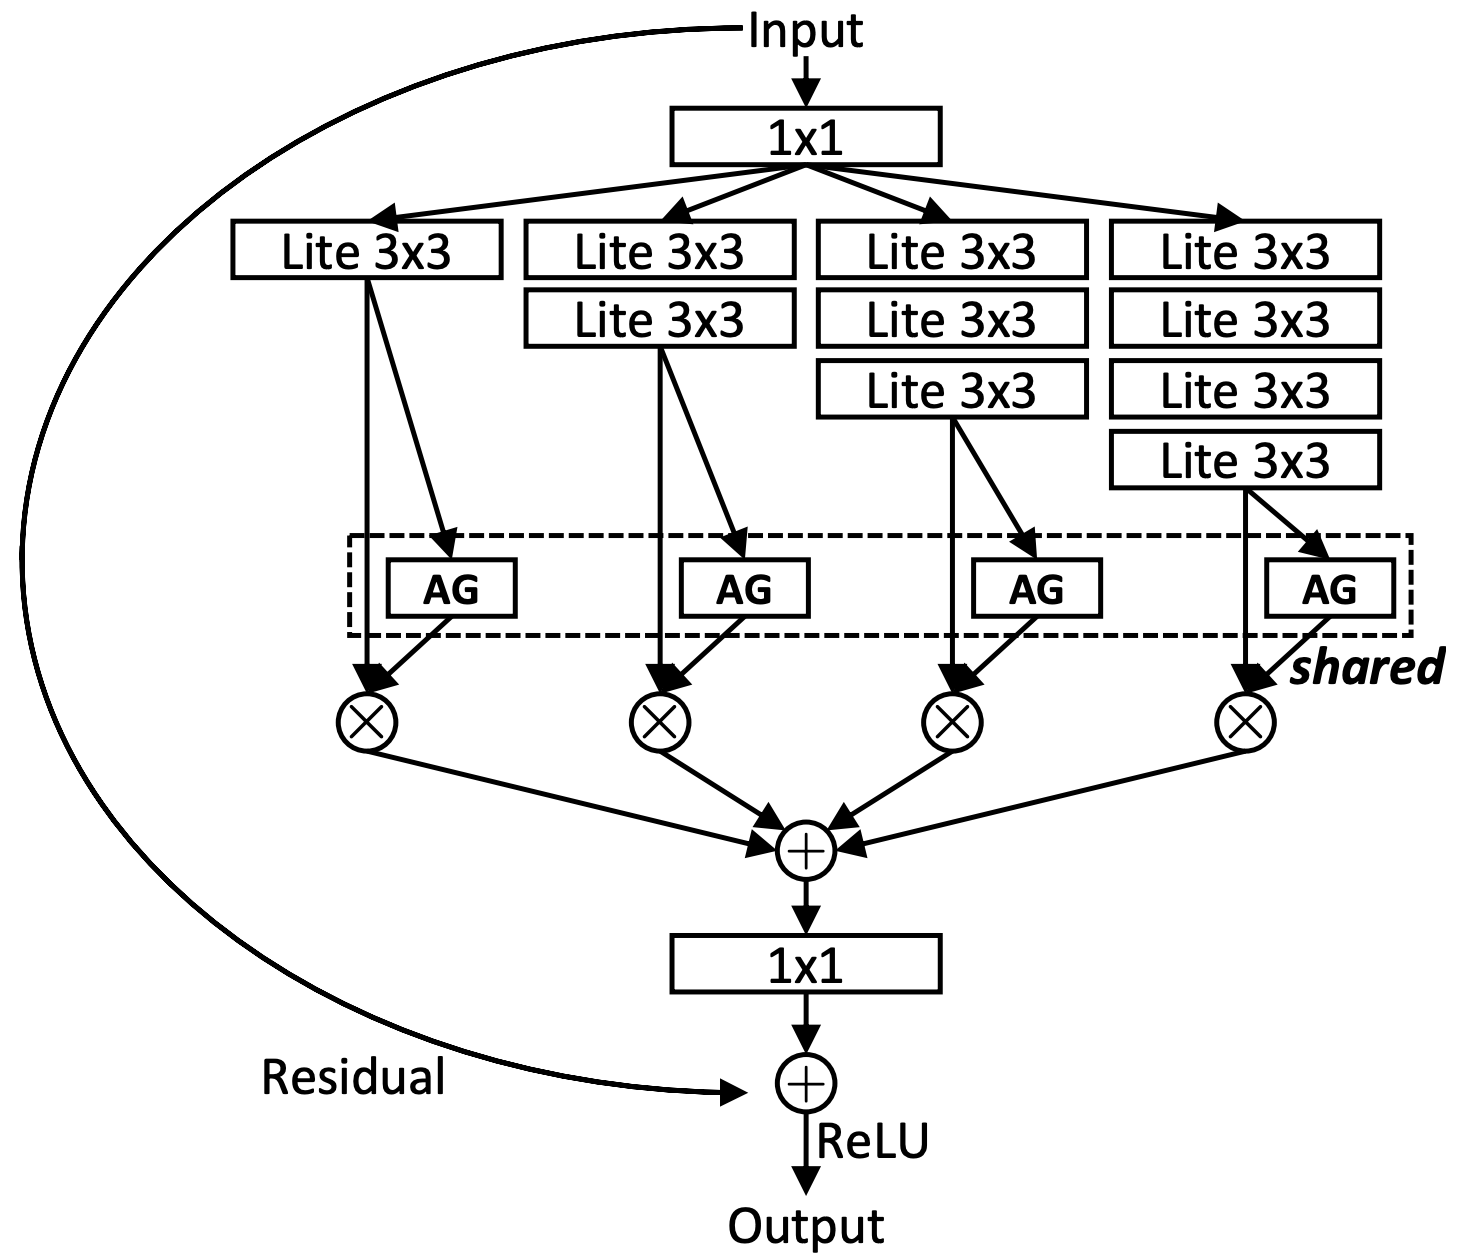
\includegraphics[width=0.95\linewidth]{OSBlock.png}
    \captionsetup{format=hang}
    \caption{Architektura bloku \emph{Bottleneck} zaprezentowana w~2019 roku przez Zhou K., Yang Y., Cavallaro A. i Xiang T. \cite{zhou}}
    \label{fig:osblock1}
\end{figure}

Sieć \emph{OSNet} została wykorzystana przez Zhou K., Yang Y., Cavallaro A. i~Xiang T. w~zadaniach związanych z~ponownym rozpoznawaniem osób na zdjęciach z~publicznego monitoringu i~uzyskała bardzo dobre wyniki, pomimo relatywnie niewielkiej liczby trenowalnych parametrów, które ta sieć posiadała. Wydaje się, iż bloki \emph{Bottleneck} zaimplementowane w~ramach sieci \emph{OSNet} mogłyby stanowić dobre uzupełnienie architektury służącej do rozpoznawania budynków na zdjęciach lotniczych, gdyż mogłyby one pomóc uzyskać odporność modelu na skalę w~jakiej prezentowane są budynki na tego typu zdjęciach.

\newpage
\subsection{Proces uczenia się głębokich sieci neuronowych}

Uczenie (trenowanie) głębokich sieci neuronowych jest najważniejszą częścią procesu ich projektowania, gdyż od jego efektywności zależy jak dobre predykcje uzyskamy z~opracowanego przez nas modelu. Może ono przyjmować kilka podstawowych form, do których najczęściej zaliczamy:

\begin{itemize}
\item uczenie nadzorowane (ang. \emph{supervised learning}) - uczenie, w którym wszystkie dane w~zbiorze uczącym mają odpowiadające im etykiety (ang. \emph{labels}), więc sieć neuronowa uczy się starając się wygenerować predykcje jak najbliższe dostępnym etykietom,
\item uczenie nienadzorowane (ang. \emph{unsupervised learning}) - uczenie, w~ramach którego dane treningowe nie mają etykiet (są nieoznaczone), więc sieć neuronowa stara się nauczyć wewnętrznej struktury danych treningowych,
\item uczenie pół-nadzorowane (ang. \emph{semi-supervised learning}) - uczenie, w~którym większość danych treningowych nie posiada etykiet, ma je tylko część danych, stanowi ono miks uczenie nadzorowanego i~nienadzorowanego,
\item uczenie ze wzmocnieniem (ang. \emph{reinforcement learning}) - uczenie, w~ramach którego oszacowany błąd służy do nakładania kar lub dawania nagród sieci neuronowej, więc sieć uczy się metodą prób i~błędów po to by zmaksymalizować zyski i~zminimalizować kary.
\end{itemize}

W~bieżącym podrozdziale skupimy się na uczeniu nadzorowanym, gdyż to właśnie uczenie zostało wykorzystane do wytrenowania opracowanej na potrzeby niniejszej pracy sieci neuronowej. Proces nadzorowanego uczenia się głębokich sieci neuronowych możemy podzielić na dwie fazy: przechodzenie danych treningowych przez sieć neuronową w~przód (ang. \emph{forward propagation}) oraz przechodzenie informacji o~wartości funkcji strat w~tył (ang. \emph{backward propagation}). W~czasie fazy przechodzenia w~przód dane treningowe są przetwarzane, warstwa po warstwie, w~taki sposób, że wszystkie neurony nakładają swoje transformacje na informacje, którą uzyskują z~poprzednich neuronów i~tak przetworzona informacja jest następnie przekazywana dalej w głąb sieci. Po przejściu przez całą sieć neuronową, ostatnia jej warstwa generuje predykcję dla konkretnego przykładu uczącego. Następnie taka predykcja, wraz z~prawidłową etykietą trafiają do, zdefiniowanej dla danej sieci, funkcji straty (ang. \emph{loss function}), która wylicza błąd tej predykcji na podstawie odpowiedniej miary podobieństwa prognozowanej przez sieć etykiety oraz rzeczywistej etykiety. Tak wyliczona wartość błędu jest następnie wstecznie propagowana do wszystkich neuronów sieci, zaczynając od neuronów znajdujących się w~warstwie końcowej aż do neuronów z~warstw początkowych. Każdy z~neuronów otrzymuje tylko fragment łącznej wartości funkcji strat, proporcjonalnie do tego jaki wkład miał konkretny neuron do wygenerowania predykcji etykiety. Po rozpropagowaniu informacji o~finalnej wartości funkcji strat po całej sieci, rozpoczyna się proces dostosowywania wag połączeń pomiędzy neuronami w~taki sposób, żeby jak najbardziej zminimalizować wartość funkcji strat. Proces ten nosi nazwę spadku wzdłuż gradientu (ang. \emph{gradient descent}) i~polega na zmianie wag sieci o~małe wartości po to by sprawdzić jak te zmiany wpłyną na finalną wartość funkcji strat - w~którym kierunku powinny one zachodzić, żeby zbliżyć się do globalnego minimum funkcji strat. 

Proces uczenia się sieci neuronowej jest dokonywany zazwyczaj na danych treningowych połączonych w~partie, które przepuszczane są przez model patria po partii w~następujących po sobie iteracjach (epokach). Stąd też \textbf{rozmiar partii} (ang. \emph{batch size}) oraz \textbf{liczba epok} (ang. \emph{number of epochs}) to jedne z~najważniejszych hiperparametrów sieci neuronowej i~od ich odpowiedniego wyboru często zależy finalna skuteczność naszego modelu. Zanim przystąpi się do trenowania głębokiej sieci neuronowej łączny zbiór danych należy podzielić na trzy rozłączne podzbiory: \textbf{zbiór treningowy} (ang. \emph{training set}), \textbf{zbiór walidacyjny} (ang. \emph{validation set}) oraz \textbf{zbiór testowy} (ang. \emph{test set}). Proporcje podziału łącznego zbioru danych na te trzy zbiory zależą wyłącznie od autora danego modelu, jednak bardzo często w~literaturze przyjmuje się następujący podział (kolejno): 70\%, 15\% i 15\%. Sieć neuronowa uczy się korzystając wyłącznie ze zbioru treningowego. Zbiór walidacyjny służy do monitorowania wyników sieci na danych z~poza zbioru treningowego oraz do odpowiedniego zmieniania hiperparametrów modelu w~taki sposób, aby uzyskiwać coraz lepsze wyniki. Wreszcie zbiór testowy pozwala na ocenę skuteczności predykcji finalnego modelu na niezależnym zbiorze danych bez obawy o~obciążenie takiej oceny przez odpowiedni dobór hiperparametrów. 

Poza właściwym podziałem zbioru danych, kolejnym istotnym elementem procesu przygotowania modelu do głębokiego uczenia jest dobór odpowiedniej \textbf{funkcji straty}. Funkcja ta wpływa bezpośrednio na efektywność treningu głębokich sieci neuronowych, stąd też na przestrzeni lat zaproponowanych zostało bardzo wiele różnych rodzajów funkcji strat, które były mniej lub bardziej efektywne w~zależności od tego do jakiego zadania i~w~ramach jakiej architektury były wykorzystywane. Do najpopularniejszych z~nich można zaliczyć:

\begin{itemize}
\item błąd średniokwadratowy (ang. \emph{Mean Square Error} / \emph{Quadratic Loss} / \emph{L2 Loss}) - jedna z~najprostszych funkcji strat, która mierzy średnią różnicę podniesioną do kwadratu pomiędzy predykcjami oszacowanymi przez sieć ($y_i$) a~oczekiwanymi wartościami~($\hat{y}_i$):
 \begin{equation}
MSE = \frac{\sum_{i=1}^{n}(y_i - \hat{y}_i)^2}{n}
\end{equation}
\item średni błąd absolutny (ang. \emph{Mean Absolute Error} / \emph{L1 Loss}) - funkcja ta mierzy średnią absolutną różnicę pomiędzy predykcjami oszacowanymi przez sieć ($y_i$) a~oczekiwanymi wartościami~($\hat{y}_i$):
 \begin{equation}
MAE = \frac{\sum_{i=1}^{n}|y_i - \hat{y}_i|}{n}
\end{equation}
\item entropia skrośna (ang. \emph{Cross-Entropy} / \emph{Log Loss}) - mierzy ona różnicę pomiędzy dwoma rozkładami prawdopodobieństwa dla danych zmiennych losowych, jej szczególnym przypadkiem jest binarna entropia skrośna (ang. \emph{Binary Cross-Entropy}), która jest uproszczeniem entropii skrośnej dla dwóch klas:
 \begin{equation}
CE = \sum_{i=1}^{n}p_i\cdot \log{\frac{1}{q_i}}
\end{equation}
\begin{equation}
BCE = -(p \cdot \log{q} + (1-p) \cdot log(1-q))
\end{equation}
\end{itemize}

W~bieżącej pracy wykorzystane zostaną jeszcze dwie inne, mniej popularne funkcje straty, ale znajdujące swoje zastosowanie w~semantycznej segmentacji obrazów:
\begin{itemize}
\item \emph{Dice Loss} - funkcja straty wywodząca się od współczynnika podobieństwa Sørensena, której zadaniem jest porównanie podobieństwa dwóch próbek, gdzie $p_i$~i~$g_i$~reprezentują pary odpowiadających sobie danych z~predykcji uzyskanej z~modelu i~ze zbioru oczekiwanych wartości:
\begin{equation}
DL  = 1 -\frac{2 \cdot \sum_{i}^{N}p_i \cdot q_i}{\sum_{i}^{N}p_{i}^{2}+\sum_{i}^{N}g_{i}^{2}}
\end{equation}
\item \emph{Lovász hinge loss} - funkcja straty, która jest gładkim rozszerzeniem współczynnika podobieństwa Jaccarda (znanego też pod nazwą \emph{Intersection over Union}) - została ona szeroko omówiona w~pracy \emph{The Lovasz Hinge: A Novel Convex Surrogate for Submodular Losses} napisanej przez Jiaqiana Yu i Matthew B. Blaschko \cite{yu}.
\end{itemize}

Duży wpływ na efektywność głębokiego uczenia ma również wybór właściwego \textbf{optymalizatora} (ang. \emph{optimizer}), czyli algorytmu poszukującego globalnego minimum funkcji strat. Większość obecnych optymalizatorów stosuje metodę spadku wzdłuż gradientu, jednak różnią się one sposobem aktualizacji wag w~kolejnych etapach uczenia, część optymalizatorów liczy gradient błędu dla pojedynczych danych treningowych, część dla całych partii, niektóre z~nich adaptują stopę uczenia do właściwości wag. Do najczęściej używanych optymalizatorów należą:

\begin{itemize}
\item \emph{Batch Gradient Descent} - najbardziej podstawowy optymalizator, który liczy gradient funkcji strat i~aktualizuje wagi sieci neuronowej dla całego zbioru treningowego co zapewnia względnie stabilną zbieżność do globalnego minimum, kosztem efektywności obliczeniowej,
\item \emph{Stochastic Gradient Descent} - optymalizator, który liczy gradient funkcji strat i~aktualizuje wagi sieci neuronowej dla każdego przykładu uczącego z~osobna, stąd też jest dużo bardziej efektywny obliczeniowo od optymalizatora \emph{BGD}, kosztem występowania dużej zmienności przy poszukiwaniu globalnego minimum,
\item \emph{Mini-Batch Gradient Descent} - optymalizator, który łączy w~sobie zalety \emph{BGD} i~\emph{SGD}, czyli efektywność obliczeniową i~względnie stabilną zbieżność do globalnego minimum -  proces liczenia gradientu i~aktualizacji wag w~\emph{MBGD} jest przeprowadzany na przypadkach uczących połączony w~niewielkich rozmiarów partie,
\item \emph{SGD} z~momentum - optymalizator, który łączy w~sobie zalety \emph{MBGD} oraz rozwiązuje najważniejszy problem wcześniej przedstawionych optymalizatorów, czyli fakt, iż mają one tendencję do zatrzymywania się w~punkcie siodłowym płaszczyzny gradientu, \emph{SGD} z~momentum rozwiązuje ten problem poprzez akumulowanie przeszłych gradientów w~celu wyliczenie wartości obecnego gradientu,
\item \emph{AdaGrad} - optymalizator, który dostosowuje stopę uczenia się do częstości występowania cech, stosuje on mniejszą stopę uczenia dla wag cech często występujących i~większą stopę uczenia dla wag cech rzadziej występujących, w~ten sposób wszystkie wagi konwergują w~podobnym tempie,
\item \emph{RMSprop} - optymalizator, który adresuje problem różnic w~wielkościach gradientów dla poszczególnymi wag modelu, poprzez zastosowanie indywidualnych kroków uczenia dla każdej wagi w~sieci neuronowej, 
\item \emph{Adam} (\emph{Adaptive Moment Estimation}) - najbardziej popularny optymalizator szeroko wykorzystywany do trenowania głębokich sieci neuronowych łączący w~sobie najważniejsze zalety optymalizatorów \emph{SGD} z~momentum (akumulowanie przeszłych wykładniczo malejących średnich gradientów) oraz \emph{RMSprop} (indywidualne kroki uczenia dla poszczególnych wag modelu),
\end{itemize}

Wraz z~wyborem optymalizatora, przed przystąpieniem do trenowania modelu, dobrze jest zdefiniować związane z~nim hiperparametry głębokiego uczenia czyli m.in.: \textbf{stopę uczenia} (ang. \emph{learning rate}), \textbf{momentum} (ang. \emph{momentum}), \textbf{spadek wagi} (ang. \emph{weight decay}), \textbf{spadek stopy uczenia} (ang. \emph{learning rate decay}). Chociaż jakość wytrenowania modelu ocenia się zazwyczaj przez pryzmat wartości funkcji straty to często w~czasie trenowania wylicza się też dodatkowe metryki, które mają za zadanie uchwycić inne istotne właściwości modelu, a~które mogą służyć do porównywania pomiędzy sobą modeli o~bardzo różnych architekturach i~funkcjach strat. W~bieżącej pracy zdefiniowano następujące dodatkowe metryki, które posłużą w~dalszej części pracy do oceny jakości modelu:
\begin{itemize}
\item ogólna dokładność (ang. \emph{Overall Accuracy}) - najprostsza miara oceny predykcji modelu definiowana jako:
\begin{equation}
OA = \frac{Liczba\ poprawnych\ predykcji}{Łączna\ liczba\ wszystkich\ predykcji} = \frac{TP + TN}{TP + FP + TN + FN}
\end{equation}
gdzie: \\
\hspace*{2em} TP - liczba wszystkich poprawnie zakwalifikowanych predykcji dodatnich, \\
\hspace*{2em} FP - liczba wszystkich niepoprawnie zakwalifikowanych predykcji dodatnich, \\
\hspace*{2em} TN - liczba wszystkich poprawnie zakwalifikowanych predykcji ujemnych, \\
\hspace*{2em} FN - liczba wszystkich niepoprawnie zakwalifikowanych predykcji ujemnych. 
\item wynik F1 (ang. \emph{F1 Score}) - miara precyzji definiowana w~zadaniach klasyfikacji binarnej jako średnia harmoniczna precyzji (ang. \emph{precision}) i~czułości (ang. \emph{recall}):
\begin{equation}
F1S =\frac{2 \cdot Precyzja \cdot Czułość}{Precyzja + Czułość}
\end{equation}
\begin{equation}
Precyzja = \frac{TP}{TP + FP}
\end{equation}
\begin{equation}
Czułość = \frac{TP}{TP + FN}\\
\end{equation}
\item współczynnik podobieństwa Jaccarda (ang. \emph{Jaccard Similarity Coefficient} / \emph{Intersection over Union}) - miara podobieństwa pomiędzy dwoma zbiorami zdefiniowana jako iloraz mocy części wspólnej tych zbiorów i~mocy sumy tych zbiorów:
\begin{equation}
IoU = \frac{|A \cap B |}{|A \cup B|}
\end{equation}
\item indeks podobieństwa strukturalnego (ang. \emph{Structural Similarity Index Measure}) - miara strukturalnego podobieństwa, które występuje pomiędzy dwoma obrazami $X$~i~$Y$:
\begin{equation}
SSIM(X, Y) = \frac{(2 \mu_X  \mu_Y + c_1) \cdot (2  \sigma_{XY} + c_2)}{(\mu^{2}_{X} + \mu^{2}_{Y} + c_1) \cdot (\sigma^{2}_{X} + \sigma^{2}_{Y} + c_2)}
\end{equation}
gdzie: \\
\hspace*{2em}$\mu_X$ - średnia z $X$, \\
\hspace*{2em}$\mu_Y$ - średnia z $Y$,\\
\hspace*{2em}$\sigma^{2}_{X}$ - wariancja $Y$,\\
\hspace*{2em}$\sigma^{2}_{Y}$ - wariancja $Y$,\\
\hspace*{2em}$\sigma_{XY}$ - kowariancja $X$ i $Y$,\\
\hspace*{2em}$c_1 = (0,01 \cdot L)^2$ - zmienna stabilizująca dzielenie ze słabym mianownikiem,\\
\hspace*{2em}$c_2 = (0,03 \cdot L)^2$ - zmienna stabilizująca dzielenie ze słabym mianownikiem,\\
\hspace*{2em}$L$ - rozpiętość tonalna wartości pikseli.\\
\end{itemize}

W~bieżącym rozdziale zarysowane zostały podstawy teoretyczne głębokiego uczenia, których znajomość jest niezbędna do efektywnej analizy dalszych rozdziałów niniejszej pracy. W kolejnym rozdziale przedstawione zostaną najważniejsze artykuły naukowe związane z~detekcją budynków na zdjęciach lotniczych i~satelitarnych, tak by czytelnik mógł się zapoznać ze specyfiką problemu, poznać najważniejsze wyzwania w~tej dziedzinie oraz zgłębić obecnie proponowane, przez świat nauki i~biznesu, rozwiązania.